\documentclass[11pt,a4paper]{article}
\usepackage{fontspec}
\setmainfont{TeX Gyre Pagella}
\setsansfont{TeX Gyre Heros}
\usepackage[margin=21mm,top=24mm,bottom=23mm,headheight=15pt]{geometry}
\usepackage{amsmath,amssymb,graphicx,booktabs,tabularx,longtable,array,enumitem}
\usepackage[table]{xcolor}
\usepackage{tikz}
\usetikzlibrary{arrows.meta,positioning,calc,fit,backgrounds,shapes.geometric}
\usepackage[most]{tcolorbox}
\usepackage{fancyhdr,titlesec,hyperref,bookmark,microtype,needspace}
\definecolor{ink}{HTML}{172F3B}
\definecolor{teal}{HTML}{176C73}
\definecolor{rust}{HTML}{AA4F2D}
\definecolor{pale}{HTML}{EDF5F4}
\definecolor{warm}{HTML}{FCF2EB}
\definecolor{muted}{HTML}{576872}
\hypersetup{colorlinks=true,linkcolor=teal,urlcolor=teal,pdftitle={Power Systems Module 3 - Complete Study Notes},pdfauthor={Sudheesh},bookmarksdepth=2}
\urlstyle{same}
\setlength{\parindent}{0pt}
\setlength{\emergencystretch}{3em}
\setlength{\parskip}{4pt plus 1pt}
\setlist{itemsep=3pt,topsep=4pt,leftmargin=1.4em}
\renewcommand{\arraystretch}{1.22}
\newcolumntype{Y}{>{\raggedright\arraybackslash}X}
\newcolumntype{L}[1]{>{\raggedright\arraybackslash}p{#1}}
\pagestyle{fancy}\fancyhf{}
\fancyhead[L]{\footnotesize\sffamily\color{muted}POWER SYSTEMS / MODULE 3}
\fancyhead[R]{\footnotesize\sffamily\color{muted}PCEOT503}
\fancyfoot[L]{\footnotesize\sffamily\color{muted}Fault analysis, relays and circuit breakers}
\fancyfoot[R]{\footnotesize\sffamily\thepage}
\renewcommand{\headrulewidth}{0.3pt}
\titleformat{\section}{\LARGE\sffamily\bfseries\color{ink}}{\thesection}{0.6em}{}
\titleformat{\subsection}{\large\sffamily\bfseries\color{teal}}{\thesubsection}{0.5em}{}
\titleformat{\subsubsection}{\normalsize\sffamily\bfseries\color{ink}}{}{0pt}{}
\titlespacing*{\section}{0pt}{12pt}{9pt}
\titlespacing*{\subsection}{0pt}{11pt}{5pt}
\titlespacing*{\subsubsection}{0pt}{8pt}{3pt}
\tcbset{enhanced,breakable,boxrule=0.4pt,arc=2pt,left=8pt,right=8pt,top=6pt,bottom=6pt,before skip=6pt,after skip=6pt,fonttitle=\sffamily\bfseries}
\newenvironment{Idea}[1]{\begin{tcolorbox}[colback=pale,colframe=teal,coltitle=white,title={#1}]}{\end{tcolorbox}}
\newenvironment{Caution}[1]{\begin{tcolorbox}[colback=warm,colframe=rust,coltitle=white,title={#1}]}{\end{tcolorbox}}
\newenvironment{Worked}[1]{\begin{tcolorbox}[breakable=false,colback=white,colframe=teal,colbacktitle=pale,coltitle=ink,title={#1}]}{\end{tcolorbox}}
\newcommand{\slides}[1]{{\small\color{muted}\textsf{Class-slide anchor: #1.}}\par}
\newcommand{\chapterstart}[2]{\clearpage\section{#1}\label{#2}}
\newcommand{\checkq}[2]{\begin{tcolorbox}[breakable=false,colback=pale,colframe=teal,coltitle=white,title={Check your understanding}]#1\par\textbf{Answer:} #2\end{tcolorbox}}
\tikzset{block/.style={draw=teal,fill=pale,rounded corners=2pt,align=center,text width=2.65cm,minimum height=1.0cm,font=\small\sffamily},hot/.style={block,draw=rust,fill=warm},arr/.style={-{Stealth[length=2.2mm]},thick,draw=ink},control/.style={arr,dashed,draw=rust}}
\newcommand{\diagramcaption}[1]{\par\smallskip{\small\color{muted}#1}\par}
\widowpenalty=10000\clubpenalty=10000
\newcommand{\ans}[1]{\boxed{#1}}
\newcommand{\phas}[2]{#1\angle #2^\circ}
\newcommand{\jj}{\mathrm j}
\begin{document}
\pagenumbering{roman}
\begin{titlepage}
\vspace*{12mm}
{\small\sffamily\color{teal}CET / SEMESTER 5 / PCEOT503}\par\vspace{16mm}
{\Huge\sffamily\bfseries\color{ink}POWER SYSTEMS}\par\vspace{6mm}
{\huge\sffamily\color{teal}Module 3}\par\vspace{10mm}
{\LARGE\sffamily Fault analysis, protective relays\\and circuit breakers}\par\vspace{14mm}
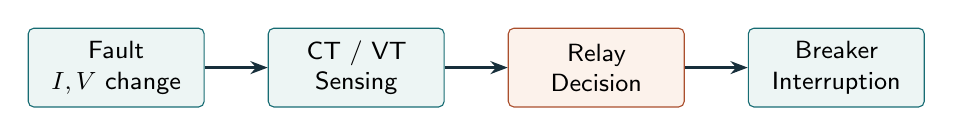
\begin{tikzpicture}[node distance=8mm]
\node[block,text width=2cm] (f) {Fault\\$I,V$ change};
\node[block,text width=2cm,right=of f] (m) {CT / VT\\Sensing};
\node[hot,text width=2cm,right=of m] (r) {Relay\\Decision};
\node[block,text width=2cm,right=of r] (b) {Breaker\\Interruption};
\draw[arr] (f)--(m);\draw[arr] (m)--(r);\draw[arr] (r)--(b);
\end{tikzpicture}\par\vspace{14mm}
\begin{Idea}{Learn the calculation and the physical response together}
Per-unit quantities; symmetrical components; sequence networks; every supplied class fault problem; protection principles; induction, static and numerical relays; and a complete syllabus supplement on arc extinction, SF$_6$ and vacuum circuit breakers.
\end{Idea}
\vfill
{\small Comprehensive study notes covering per-unit systems, symmetrical components, fault analysis, protective relaying, and circuit breakers according to the 2024-scheme syllabus.}\par\vspace{4mm}
{\small\sffamily Prepared for Sudheesh / 8 October 2026}
\end{titlepage}
\tableofcontents\clearpage\pagenumbering{arabic}

\chapterstart{Study map and notation}{map}
\subsection{Everything required by the supplied Module 3 syllabus}
Module 3 has 11 contact hours and combines analysis with protection. The analysis predicts currents and voltages during faults; protection uses measurements to decide which breakers should interrupt those currents.
\begin{center}\small
\begin{tabularx}{\textwidth}{L{.38\textwidth}Y}
\toprule Syllabus item & What this note develops\\\midrule
Per-unit quantities: single and three phase & Base definitions, change of base, transformer referral, complete class examples.\\
Symmetrical components and sequence networks & Forward/inverse transformations, phasor sets, component models, grounding and transformer zero-sequence paths.\\
Fault types and shunt-fault calculations & Three-phase, LG, LL and LLG boundary-condition derivations; solid and finite-impedance faults; every supplied class numerical. Series/open-conductor fault calculations are outside scope.\\
Need for protection; primary and backup & Selectivity, reliability, stability, sensitivity, speed, zones, coordination and breaker failure.\\
Induction-type electromechanical relay & Construction, phase-displaced flux, torque, disc/cup structures, pickup and time settings.\\
Static OC and instantaneous OC & Labelled functional block diagrams, comparators, timing and trip chain.\\
Microprocessor OC; numerical relay & Hardware diagram, flowchart, sampling, digital estimation, timing, functions and limitations.\\
OC, directional, distance, differential & Measured quantities, decision principles, applications, characteristic sketches and examples.\\
Circuit breaker; arc; extinction principles/methods & Contact separation, current zero, recovery voltage, thermal/dielectric recovery, high/low-resistance methods.\\
SF$_6$ and VCB & Construction, interruption sequence, advantages/limitations and comparison.\\\bottomrule
\end{tabularx}\end{center}
\begin{Caution}{Key analytical pitfalls to avoid}
In unsymmetrical fault analysis, double-line-to-ground (LLG) calculations require strict adherence to sequence current sign conventions to ensure zero fault current in the unfaulted phase ($I_a=0$). Section~\ref{faultnumericals} works through the complete boundary conditions and verification checks.
\end{Caution}

\Needspace{95mm}
\subsection{Notation and assumptions used throughout}
\begin{itemize}
\item $a=e^{\jj120^\circ}$ is the \emph{sequence rotation operator}, not a transformer turns ratio. Use $t=N_H/N_L$ for the latter.
\item Sequence ordering is $(0,1,2)$: zero, positive, negative. $V_1$ means the phase-$a$ positive-sequence voltage; the other two phases follow by rotation. $I_k$ has the same convention.
\item $E$ is the pre-fault positive-sequence Thevenin phase voltage at the fault bus. $Z_1,Z_2,Z_0$ are the driving-point sequence impedances seen there on a common base. They are not automatically the reactance of just one generator.
\item Fault currents are directed from the network \emph{into the fault}. We analyse an $a$-ground fault, a $b$-$c$ fault and a $b$-$c$-ground fault. Relabelling phases changes phasors, not the method.
\item Unless stated otherwise: balanced pre-fault network, $E=1\angle0^\circ$ p.u., no pre-fault load-current contribution, balanced sequence-decoupled equipment, and RMS phasors. Reactance-only examples neglect resistance. These are textbook calculation assumptions.
\end{itemize}
\checkq{Why is a fault calculation not enough to design protection?}{It predicts electrical stresses under a stated network model. Relay decisions also need operating settings, selectivity, instrument-transformer performance, breaker clearing capability and contingency/backup analysis.}

\chapterstart{Per-unit quantities without hidden factors}{pu}
\slides{Per-unit part pp. 1--16}
\subsection{The idea: normalise quantities to a consistent base}
\[
 x_{\rm pu}=\frac{x_{\rm actual}}{x_B},\qquad x_{\rm actual}=x_{\rm pu}x_B,\qquad x_{\%}=100x_{\rm pu}.
\]
A reactance of 20\% is $0.2$ p.u. on the base for which it was specified. ``Per unit'' has no unit, but it is meaningless without its base. $0.2$ p.u. on 10 MVA and $0.2$ p.u. on 100 MVA are not the same physical impedance if the voltage bases match.

A network has machines, transformers and lines at different voltage levels. Ohmic impedances must be referred across every transformer before direct combination. Per-unit values avoid repeated referral \emph{after} we choose consistent bases. Apparatus ratings and typical p.u. reactances also become easier to compare.
\subsection{Single-phase base quantities}
Choose base apparent power $S_B$ and RMS voltage $V_B$ independently. Then
\[
 S_B=V_B I_B,\qquad I_B=\frac{S_B}{V_B},\qquad
 Z_B=\frac{V_B}{I_B}=\frac{V_B^2}{S_B},\qquad Y_B=\frac1{Z_B}.
\]
With $S_B$ in kVA and $V_B$ in kV:
\[
 I_B=\frac{S_B(\mathrm{kVA})}{V_B(\mathrm{kV})}\ \mathrm A,\qquad
 Z_B=\frac{1000V_B^2(\mathrm{kV})}{S_B(\mathrm{kVA})}\ \Omega.
\]
A genuine single-phase circuit uses its own terminal voltage and total single-phase VA. A one-phase equivalent of a balanced three-phase system uses phase voltage and one-third of total VA. These are two applications of the same formula; single phase does not inherently imply a line-to-neutral connection.
\subsection{Three-phase bases and the cancellation of square root three}
Use total three-phase $S_B$ and line-to-line voltage magnitude $V_{B,LL}$. The phase equivalent has
\[
 S_{B,\rm phase}=S_B/3,\qquad V_{B,\rm phase}=V_{B,LL}/\sqrt3.
\]
Therefore
\[
 \ans{I_B=\frac{S_B}{\sqrt3V_{B,LL}}},\qquad
 \ans{Z_B=\frac{(V_{B,LL}/\sqrt3)^2}{S_B/3}=\frac{V_{B,LL}^2}{S_B}}.
\]
$Z_B$ is the \emph{per-phase equivalent impedance base}. Convenient engineering forms are
\[
 I_B(\mathrm{kA})=\frac{S_B(\mathrm{MVA})}{\sqrt3V_{B,LL}(\mathrm{kV})},\quad
 Z_B(\Omega)=\frac{V_{B,LL}^2(\mathrm{kV})}{S_B(\mathrm{MVA})}.
\]
Using kVA/kV instead gives current in amperes and requires the factor 1000 in $Z_B$. Do not insert another $\sqrt3$ into the impedance formula. For a physical delta-connected branch impedance, first convert to its star phase equivalent or explicitly define delta-branch bases; the network's standard per-phase $Z_B$ is not a declaration that every winding is physically star connected.

For consistent phase-reference phasors in a balanced system,
\[
 S_{\rm pu}=V_{\rm pu}I_{\rm pu}^*,\qquad V_{\rm pu}=Z_{\rm pu}I_{\rm pu}.
\]
Here $S_{\rm pu}$ is total three-phase complex power divided by total $S_B$; $V_{\rm pu}$ uses phase voltage divided by its phase base. The phase/line \emph{magnitudes} have the same p.u. value. Their phasor reference angles need attention: $V_{ab}$ is displaced by $30^\circ$ from $V_a$ in positive sequence.

\subsection{Derive change of base rather than memorising its direction}
The physical impedance stays the same:
\[
 Z_{\rm actual}=Z_{\rm pu,old}\frac{V_{B,old}^2}{S_{B,old}}.
\]
Divide by the new base impedance:
\[
 \ans{Z_{\rm pu,new}=Z_{\rm pu,old}
 \frac{S_{B,new}}{S_{B,old}}
 \left(\frac{V_{B,old}}{V_{B,new}}\right)^2}.
\]
Voltage bases must refer to the same physical side when using this formula directly. Increasing base MVA increases p.u. impedance; increasing base voltage decreases it quadratically. A p.u. impedance can be complex; apply the real base multiplier to both $R$ and $X$.

\subsection{Why an ideal transformer disappears from a p.u. diagram}
Let $t=N_H/N_L=V_H/V_L$ for a single-phase ideal transformer. Current magnitudes obey $I_L=tI_H$. Equal physical loss and reactive-power effect require
\[
 Z_H=t^2Z_L.
\]
With common $S_B$ and $V_{B,H}=tV_{B,L}$,
\[
 Z_{B,H}=t^2Z_{B,L},\qquad
 \frac{Z_H}{Z_{B,H}}=\frac{t^2Z_L}{t^2Z_{B,L}}=\frac{Z_L}{Z_{B,L}}.
\]
Thus the transformer leakage impedance has the same p.u. value on both sides. It remains in the equivalent diagram; the \emph{ideal ratio element} can be removed. For three-phase transformers, propagate line-voltage bases using the rated line-voltage ratio, which includes connection effects; do not automatically substitute a winding turns ratio for it. Vector-group phase shifts and zero-sequence connections still matter in their appropriate studies.

\subsubsection{Transformer equivalent}\slides{Per-unit, p. 14}
\begin{center}\includegraphics[width=.94\textwidth,height=68mm,keepaspectratio]{Study_Assets/Module3/pu_014.pdf}\end{center}
\diagramcaption{The ideal turns ratio disappears only with consistent voltage bases on the two sides. Leakage impedance remains.}

\subsubsection{Referred impedance}\slides{Per-unit, p. 15}
\begin{center}\includegraphics[width=.94\textwidth,height=68mm,keepaspectratio]{Study_Assets/Module3/pu_015.pdf}\end{center}
\diagramcaption{A single per-unit series impedance can replace the referred transformer equivalent.}
\begin{Idea}{A reliable base-selection workflow}
Choose one system MVA base. Choose voltage base at one bus. Propagate voltage bases through transformer rated voltage ratios. Calculate each local $Z_B,I_B$. Convert every nameplate or ohmic impedance to that local common base. Then draw the impedance/sequence network and combine values. At the end, multiply p.u. current by the base current \emph{at the fault bus}.
\end{Idea}

\chapterstart{Every per-unit class example}{puexamples}
\subsection{20 kVA single-phase transformer: 2000/200 V}
\slides{Per-unit part pp. 10--15}
Leakage $X=0.8\ \Omega$ referred to the 200 V side:
\[
 Z_{B,L}=\frac{200^2}{20000}=2\ \Omega,\qquad
 \ans{X_{\rm pu}=0.8/2=0.4\ \mathrm{p.u.}=40\%}.
\]
On the HV side $t=10$, so $X_H=0.8(10)^2=80\ \Omega$ and $Z_{B,H}=2000^2/20000=200\ \Omega$. Again $80/200=0.4$ p.u. The large p.u. value is the given arithmetic; do not replace it by a guessed typical reactance.
\subsection{Class Example 2.6: line impedance on 100 MVA, 132 kV}
\slides{Per-unit part pp. 17--18}
For $Z=30+\jj110\ \Omega$/phase,
\[
 Z_B=132^2/100=174.24\ \Omega,\qquad
 \ans{Z_{\rm pu}=0.172176+\jj0.631313}.
\]
The source's $0.172+\jj0.631$ is this result rounded. Base voltage is line-to-line and MVA is total three-phase; $Z$ is per phase.
\subsection{Class Example 2.7: generator reactance on a new base}
\slides{Per-unit part pp. 19--20}
Given generator rating 30 MVA, 11 kV and $X_{old}=0.2$ p.u.; requested base 50 MVA, 33 kV:
\[
 \ans{X_{new}=0.2\frac{50}{30}\left(\frac{11}{33}\right)^2
 =0.037037\ \mathrm{p.u.}}.
\]
This is a change to an arbitrarily requested voltage base \emph{on the same physical side}. It does not claim the generator physically operates at 33 kV. If an actual 11/33 kV transformer were being crossed with bases following its ratio, the p.u. generator reactance would remain unchanged by that crossing, apart from any MVA-base change. Confirm by ohms: $X=0.2(11^2/30)=0.806667\ \Omega$, new $Z_B=33^2/50=21.78\ \Omega$.
\Needspace{105mm}
\subsection{Balanced system: 30 MVA, 12 kV, given impedance}
\slides{Per-unit part pp. 21--24}
Given apparent-power magnitude $S=30$ MVA, $V_{LL}=12$ kV and $Z=1.5+\jj2\ \Omega$/phase; initial bases 50 MVA, 10 kV:
\[
 I_B=\frac{50}{\sqrt3(10)}=2.886751\ \mathrm{kA},\quad Z_B=10^2/50=2\ \Omega,
\]
\[
 \ans{|V_{\rm pu}|=1.2},\quad |I|=\frac{30}{\sqrt3(12)}=1.443376\ \mathrm{kA},\quad
 \ans{|I_{\rm pu}|=0.5},\quad \ans{Z_{\rm pu}=0.75+\jj1.0}.
\]
$|Z_{\rm pu}|=1.25$. On 100 MVA, 20 kV,
\[
 \ans{Z_{\rm pu,new}=(0.75+\jj1)\frac{100}{50}\left(\frac{10}{20}\right)^2
 =0.375+\jj0.5}.
\]
New $Z_B=4\ \Omega$, providing the direct check $(1.5+\jj2)/4$.
\begin{Caution}{Do not infer more than these data specify}
No power factor is given, so the current result is a \emph{magnitude}, not a fully known phasor. The supplied impedance cannot also be the sole load impedance consuming the stated 30 MVA at 12 kV: that would require $|Z_{load}|=V_{LL}^2/|S|=4.8\ \Omega$, rather than 2.5 $\Omega$. Treat $Z$ as separately supplied component/network impedance. This avoids a false attempt to force $V/I=Z$ for unrelated quantities.
\end{Caution}

\chapterstart{Symmetrical components: what the transform means}{sequence}
\slides{Symmetrical-components part pp. 1--15, 26}
\subsection{Decompose an unbalanced set into three simple patterns}
Any three phase phasors at the \emph{same frequency} can be uniquely written as a sum of positive-, negative- and zero-sequence sets. This is an algebraic decomposition, not three physically separate power systems. Independent sequence circuits are obtained only when the underlying linear network is sequence decoupled, as in the usual balanced/transposed model.

Positive sequence has equal magnitudes, $120^\circ$ separation and phase order $a$-$b$-$c$. Negative sequence has equal magnitudes, $120^\circ$ separation and order $a$-$c$-$b$. Zero sequence has three identical, in-phase phasors; it is symmetric but is not a $120^\circ$ balanced rotating set.
\begin{center}
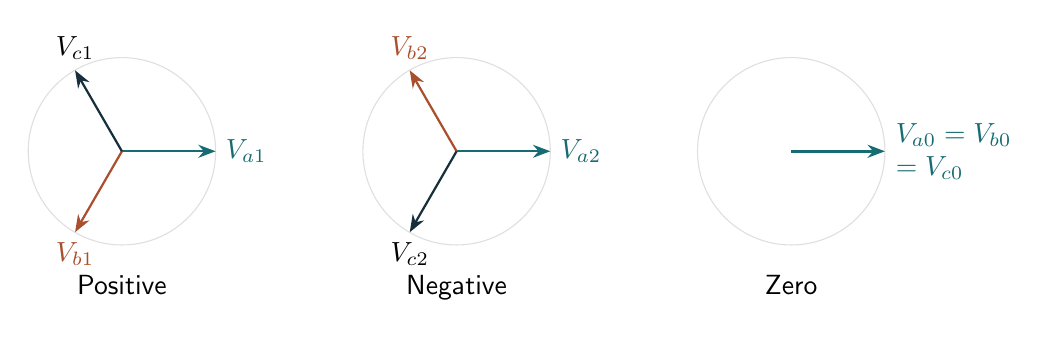
\begin{tikzpicture}[scale=.85]
\foreach \x/\t in {0/Positive,5/Negative,10/Zero}{\draw[gray!25] (\x,0)circle(1.4);\node[below] at (\x,-1.7){\sffamily\t};}
\draw[arr,teal] (0,0)--(1.4,0)node[right]{$V_{a1}$};
\draw[arr,rust] (0,0)--(-.7,-1.21)node[below]{$V_{b1}$};
\draw[arr] (0,0)--(-.7,1.21)node[above]{$V_{c1}$};
\draw[arr,teal] (5,0)--(6.4,0)node[right]{$V_{a2}$};
\draw[arr,rust] (5,0)--(4.3,1.21)node[above]{$V_{b2}$};
\draw[arr] (5,0)--(4.3,-1.21)node[below]{$V_{c2}$};
\draw[arr,teal,very thick] (10,0)--(11.4,0)node[right,align=left]{$V_{a0}=V_{b0}$\\$=V_{c0}$};
\end{tikzpicture}
\end{center}

\subsubsection{An unbalanced phasor set}\slides{Sequence, p. 5}
\begin{center}\includegraphics[width=.94\textwidth,height=68mm,keepaspectratio]{Study_Assets/Module3/seq_005.pdf}\end{center}
\diagramcaption{Unequal magnitudes or unequal angular separations require component decomposition.}

\subsubsection{Three sequence phasor sets}\slides{Sequence, p. 6}
\begin{center}\includegraphics[width=.94\textwidth,height=68mm,keepaspectratio]{Study_Assets/Module3/seq_006.pdf}\end{center}
\diagramcaption{Read the phase labels: positive a-b-c, negative a-c-b, zero all coincident. The main text fixes a=1 angle 120 degrees.}
Define
\[
 a=-\tfrac12+\jj\tfrac{\sqrt3}{2},\quad a^2=-\tfrac12-\jj\tfrac{\sqrt3}{2},\quad
 a^3=1,\quad 1+a+a^2=0,\quad a^{-1}=a^2.
\]
Multiplication by $a$ rotates a phasor $120^\circ$ anticlockwise. Positive sequence obeys $V_{b1}=a^2V_1$, $V_{c1}=aV_1$; negative sequence obeys $V_{b2}=aV_2$, $V_{c2}=a^2V_2$. These relations fix the signs and positions in the matrices.

\subsection{From sequence quantities back to actual phase quantities}
Each phase is the sum of its three component contributions:
\[
 V_a=V_0+V_1+V_2,\quad V_b=V_0+a^2V_1+aV_2,\quad
 V_c=V_0+aV_1+a^2V_2.
\]
Thus
\[
 \ans{\begin{bmatrix}V_a\\V_b\\V_c\end{bmatrix}=
 \underbrace{\begin{bmatrix}1&1&1\\1&a^2&a\\1&a&a^2\end{bmatrix}}_{T}
 \begin{bmatrix}V_0\\V_1\\V_2\end{bmatrix}}.
\]
The same transform applies to currents and other three-phase phasor sets. Always state the sequence-vector order; textbooks also use $(1,2,0)$, which rearranges the matrix.
\subsection{Derive the inverse transformation}
Add the three phase equations. Since $1+a+a^2=0$, the positive and negative contributions cancel, leaving $V_a+V_b+V_c=3V_0$. Similarly, $V_a+aV_b+a^2V_c=3V_1$ and $V_a+a^2V_b+aV_c=3V_2$.
\[
 \ans{\begin{bmatrix}V_0\\V_1\\V_2\end{bmatrix}=\frac13
 \begin{bmatrix}1&1&1\\1&a&a^2\\1&a^2&a\end{bmatrix}
 \begin{bmatrix}V_a\\V_b\\V_c\end{bmatrix}}.
\]
Verify $T^{-1}T=I$ using $a^3=1$ and $1+a+a^2=0$. In a balanced positive-sequence set, only $V_1$ remains. A reverse balanced set has only $V_2$; equal in-phase phasors have only $V_0$. An arbitrary unbalanced set need not contain all three: a three-wire set with zero current sum has $I_0=0$ even when unbalanced.

\subsection{Physical consequences that make the decomposition useful}
\[
 I_a+I_b+I_c=3I_0.
\]
If phase currents are all referenced outward from a bus, the return-path current balances this sum with the appropriate opposite sign. Zero-sequence current therefore needs a return path: neutral, earth, another conductor, or circulating winding paths as allowed by the equipment. It is not limited to physical earth. Zero-sequence \emph{voltage} can exist without a conducting earth-current path, as in neutral displacement.

Line-to-line voltage cancels zero sequence: $V_{ab}=V_a-V_b$. Consequently zero-sequence voltage cannot be recovered from just line-to-line voltages; phase-to-reference information is needed. A balanced positive-sequence generator produces no negative/zero internal EMF in the elementary model, yet these \emph{currents} can flow during faults because the fault conditions connect the networks and the positive source drives them.

An ideal symmetrical-component power identity, useful as a check, is
\[
 S_{3\phi}=V_aI_a^*+V_bI_b^*+V_cI_c^*
 =3(V_0I_0^*+V_1I_1^*+V_2I_2^*).
\]
For a rotating machine, negative-sequence currents produce a reverse rotating stator field, seen at twice synchronous electrical frequency by its rotor, causing heating. This explains why unbalance can be damaging even without a very large positive-sequence current. Converter-connected sources may have controls and current limits that require a more detailed model than a fixed EMF behind reactance.

\chapterstart{All five class symmetrical-component examples}{sequenceexamples}
\subsection{Balanced normal phase order}
\slides{Symmetrical-components part pp. 16--17}
$V_a=100\angle0^\circ$, $V_b=100\angle-120^\circ=100a^2$, $V_c=100\angle120^\circ=100a$ V:
\[
 V_0=\tfrac{100}{3}(1+a^2+a)=0,\quad
 V_1=\tfrac{100}{3}(1+a^3+a^3)=100,\quad
 V_2=\tfrac{100}{3}(1+a+a^2)=0.
\]
\[
 \ans{V_0=0,\quad V_1=100\angle0^\circ\ \mathrm V,\quad V_2=0}.
\]
\subsection{Balanced reverse phase order}
\slides{Symmetrical-components part pp. 18--19}
Now $V_a=100$, $V_b=100a$, $V_c=100a^2$ V. Substitute into the inverse transform:
\[
 \ans{V_0=0,\quad V_1=0,\quad V_2=100\angle0^\circ\ \mathrm V}.
\]
This is balanced negative sequence, not a mixed set merely because it has reverse order.
\subsection{Three identical in-phase voltages}
\slides{Symmetrical-components part pp. 20--21}
$V_a=V_b=V_c=60\angle0^\circ$ V. Hence $V_0=(60+60+60)/3=60$, while $V_1$ and $V_2$ vanish through $1+a+a^2=0$:
\[
 \ans{V_0=60\angle0^\circ\ \mathrm V,\quad V_1=V_2=0}.
\]
Line-to-line voltages are all zero, despite nonzero phase-to-reference voltages.
\subsection{Unequal phase magnitudes}
\slides{Symmetrical-components part pp. 22--23}
$V_a=100$, $V_b=80a^2$, $V_c=60a$ V. Convert to rectangular form or simplify the rotations algebraically:
\begin{align*}
 V_0&=\tfrac13(100+80a^2+60a)=10-\jj5.77350,\\
 V_1&=\tfrac13(100+80+60)=80,\\
 V_2&=\tfrac13(100+80a+60a^2)=10+\jj5.77350.
\end{align*}
\[
 \ans{V_0=11.5470\angle-30^\circ\ \mathrm V,\quad V_1=80\angle0^\circ\ \mathrm V,
 \quad V_2=11.5470\angle30^\circ\ \mathrm V}.
\]
Check phase $a$: $(10-\jj5.7735)+80+(10+\jj5.7735)=100$. Check the other two by the forward transformation; cancellation in phase $a$ alone is insufficient to validate the entire set.
\subsection{Given sequence currents, recover phase currents}
\slides{Symmetrical-components part pp. 24--25}
$I_0=2$, $I_1=10$, $I_2=4$ A, all at zero degrees:
\[
 I_a=2+10+4=16,\quad I_b=2+10a^2+4a=-5-\jj5.19615,
\]
\[
 I_c=2+10a+4a^2=-5+\jj5.19615.
\]
\[
 \ans{I_a=16\angle0^\circ\ \mathrm A},\quad
 \ans{I_b=7.21110\angle-133.898^\circ\ \mathrm A},\quad
 \ans{I_c=7.21110\angle133.898^\circ\ \mathrm A}.
\]
Current sum is 6 A $=3I_0$, not zero. A physical implementation needs a permitted return path for that current.

\chapterstart{Build sequence networks from real equipment}{networks}
\slides{Symmetrical-components part pp. 9--11, 14--15; fault-analysis part pp. 7--11}

\subsubsection{One-line symbol key}\slides{Fault, p. 9}
\begin{center}\includegraphics[width=.94\textwidth,height=68mm,keepaspectratio]{Study_Assets/Module3/fault_009.pdf}\end{center}
\diagramcaption{Recognize generator, bus, transformer, circuit breaker, transmission line and load before drawing equivalent networks.}

\subsubsection{A class one-line system}\slides{Fault, p. 8}
\begin{center}\includegraphics[width=.94\textwidth,height=68mm,keepaspectratio]{Study_Assets/Module3/fault_008.pdf}\end{center}
\diagramcaption{Generator, transformers, line, breakers, buses and load are represented by one phase of a balanced three-phase network.}
\subsection{The three fault-bus equivalents}
For a balanced pre-fault system reduced to the fault bus,
\[
 \ans{V_1=E-Z_1I_1},\qquad \ans{V_2=-Z_2I_2},\qquad \ans{V_0=-Z_0I_0}.
\]
The minus signs follow the current direction into the fault. They are essential in LL/LLG calculations. Networks 2 and 0 have no independent internal source under the stated balanced-source model.
\begin{center}
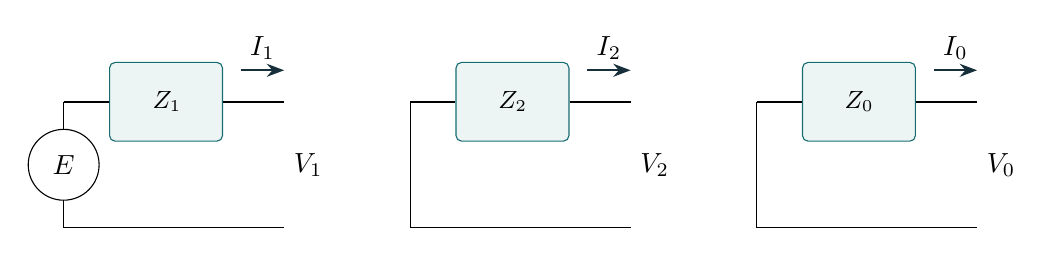
\begin{tikzpicture}
\foreach \x/\z/\i/\v in {0/Z_1/I_1/V_1,4.4/Z_2/I_2/V_2,8.8/Z_0/I_0/V_0}{
\node[block,text width=1.2cm] (z\i) at (\x+1.6,1) {$\z$};
\draw[thick] (\x+.3,1)--(z\i.west);\draw[thick] (z\i.east)--(\x+3.1,1);
\draw[arr] (\x+2.55,1.4)--(\x+3.1,1.4)node[midway,above]{$\i$};
\node[right] at (\x+3.1,.2){$\v$};\draw (\x+.3,-.6)--(\x+3.1,-.6);
}
\draw (0.3,1)--(.3,.65);\draw (.3,.2)circle(.45);\node at (.3,.2){$E$};\draw (.3,-.25)--(.3,-.6);
\draw (4.7,1)--(4.7,-.6);\draw (9.1,1)--(9.1,-.6);
\end{tikzpicture}
\end{center}
\diagramcaption{Functional Thevenin equivalents. Bottom nodes are sequence reference nodes. A drawn reference is not itself proof that a physical zero-sequence earth-return path exists.}

\subsection{Generator models and neutral impedance}
Positive sequence uses internal EMF behind an appropriate reactance. Initially after a short circuit, use subtransient $X_d''$ if specified; later use transient $X_d'$ or synchronous $X_d$ for the corresponding time interval. The AC current envelope generally decays through these stages. Resistance and an inception-dependent decaying DC offset are omitted in elementary symmetrical RMS phasor calculations; the first asymmetrical peak is not just $\sqrt2$ times a steady-state fault current.

Negative sequence uses $Z_2$ with no balanced-source internal EMF. For a machine it need not equal $Z_1$; use the given data. Zero sequence uses $Z_{0,G}$ and the actual neutral connection. If neutral-to-earth impedance is $Z_n$, zero-sequence phase currents are equal and neutral current has magnitude/phasor sum $3I_0$. Its voltage drop is $3Z_nI_0$, so the per-phase zero network contains
\[
 \ans{Z_{0,\rm branch}=Z_{0,G}+3Z_n}.
\]
An ungrounded neutral blocks the simple conductive zero-sequence branch, but actual networks may still have capacitive earth paths. Do not count $3Z_n$ twice if the supplied $Z_0$ already includes neutral grounding.
\subsection{Lines and transformers}
A balanced/transposed line usually has $Z_2=Z_1$ in the elementary model. Its $Z_0$ is different because same-phase zero-sequence currents return through earth/neutral and link different magnetic paths. Use measured/given zero-sequence data rather than guessing $Z_0=Z_1$.

A transformer has approximately equal positive and negative leakage sequence impedances in the usual model; vector groups can introduce opposite phase shifts in the two sequences. Zero-sequence behaviour depends on winding connections, neutral grounding, magnetic core construction and external paths.
\begin{center}\small
\begin{tabularx}{\textwidth}{L{.29\textwidth}Y}
\toprule Connection & Elementary zero-sequence line-current behaviour\\\midrule
Grounded star / delta & Grounded-star side can support zero-sequence line current with corresponding delta circulation. It cannot appear as zero-sequence \emph{line current} on the delta side.\\
Ungrounded star & No conductive neutral return in the elementary model: external zero-sequence line-current path is open.\\
Delta & Zero-sequence winding currents may circulate internally. Equal zero-sequence components cancel in delta line currents.\\
Grounded star / grounded star & Zero-sequence transfer may be possible when both returns and the transformer magnetic path permit it. Include neutral impedances and the specified zero-sequence transformer model.\\\bottomrule
\end{tabularx}\end{center}
For a delta, line current is the difference of adjacent winding currents. Equal circulating components give $I_{a0,\rm line}=I_{ab0}-I_{ca0}=0$, while winding current can remain nonzero. Saying ``delta blocks zero sequence'' is acceptable only if you mean zero-sequence current \emph{in its external lines}.

\subsection{Reduce the network at the fault bus}
Deactivate independent voltage sources to compute sequence driving-point impedances, preserving their internal impedance. Combine series/parallel paths on the common base. Preserve connection-dependent zero-sequence topology. For a multi-bus study, network inversion or a bus-impedance matrix can provide the driving-point element; simple class examples are already reduced.
\begin{Worked}{Additional example: grounding changes only the required branch}
A star generator has $Z_1=\jj0.2$, $Z_2=\jj0.2$, $Z_{0,G}=\jj0.1$ p.u. and neutral reactance $Z_n=\jj0.05$ p.u. Its positive/negative values remain $\jj0.2$; its effective zero-sequence branch becomes $\jj(0.1+3\times0.05)=\jj0.25$. A solid LG fault gives $I_a=3/(\jj0.65)=-\jj4.61538$ p.u., compared with $-\jj6$ for solid neutral grounding. A three-phase fault remains $I_a=1/(\jj0.2)=-\jj5$ p.u. in this model.
\end{Worked}

\chapterstart{Derive each shunt-fault connection}{faults}
\slides{Fault-analysis part pp. 1--18}
\subsection{Fault types, causes and consequences}
A shunt fault makes an unintended conducting path between phases and/or to earth. Causes include insulation deterioration, lightning/overvoltage flashover, damaged equipment, contamination, vegetation/animals and mechanical/human error. Arcing and high-resistance faults need not be literal metal-to-metal contact or an extreme current surge. They still can create dangerous conditions.

Balanced three-phase faults (LLL, or balanced LLLG) are symmetrical. LG, LL and LLG are unsymmetrical. Open-conductor/series faults are another category, recognised here but not calculated because the syllabus specifies shunt calculations only. Short circuits can heat and mechanically stress equipment, depress voltage, endanger people and disrupt stability. Analysis supports breaker-duty selection and protection studies.
\begin{Caution}{Do not rank every fault by a universal severity rule}
A three-phase fault is a common reference for breaker duty, but it is not always the highest current. A solid LG fault can exceed it if zero-sequence impedance is sufficiently low. The actual network, grounding and fault impedance determine the result.
\end{Caution}

\subsection{Balanced three-phase fault: positive sequence only}
For equal phase fault impedances $Z_f$, the fault is balanced; $I_0=I_2=0$. Phase-$a$ boundary condition is $V_a=Z_fI_a$. Since $V_a=V_1$ and $I_a=I_1$,
\[
 E-Z_1I_1=Z_fI_1\quad\Rightarrow\quad
 \ans{I_1=\frac{E}{Z_1+Z_f}},\qquad
 I_a=I_1,\ I_b=a^2I_1,\ I_c=aI_1.
\]
For a solid fault $Z_f=0$ and the fault phase voltages are zero in the ideal model. A balanced LLL fault without earth has the same positive-sequence result; no zero sequence is generated just by adding a balanced ground connection.

\subsection{Single-line-to-ground fault on phase a}
At the fault point, unfaulted-branch currents are $I_b=I_c=0$, while $V_a=Z_fI_a$. Apply the inverse current transform:
\[
 I_0=I_1=I_2=I_a/3.
\]
Add the three sequence voltages:
\[
 V_a=V_0+V_1+V_2=E-(Z_1+Z_2+Z_0)I_1=3Z_fI_1.
\]
Thus
\[
 \ans{I_0=I_1=I_2=\frac{E}{Z_1+Z_2+Z_0+3Z_f}},\qquad
 \ans{I_a=\frac{3E}{Z_1+Z_2+Z_0+3Z_f}}.
\]
The three sequence impedances and $3Z_f$ are in series. $Z_f$ is the phase-to-earth fault impedance, not a neutral impedance; both may appear in the same problem, in different places. Fault-branch $I_b=I_c=0$ does not mean all upstream load currents are zero in a loaded network.

\subsubsection{LG series connection}\slides{Fault, p. 14}
\begin{center}\includegraphics[width=.94\textwidth,height=68mm,keepaspectratio]{Study_Assets/Module3/fault_014.pdf}\end{center}
\diagramcaption{All three sequence currents are equal. Neutral impedance 3Zn belongs inside Z0; the external phase fault appears as 3Zf, counted separately.}

\subsubsection{Finite-impedance LG network}\slides{Fault, p. 25}
\begin{center}\includegraphics[width=.94\textwidth,height=68mm,keepaspectratio]{Study_Assets/Module3/fault_025.pdf}\end{center}
\diagramcaption{The return branch is 3Zf because the physical phase current is three times the sequence current.}

\subsection{Line-to-line fault between b and c}
With impedance $Z_f$ between the two phases,
\[
 I_a=0,\quad I_b=-I_c,\quad V_b-V_c=Z_fI_b.
\]
There is no return current, so $I_0=0$; then $I_2=-I_1$. From the transform,
\[
 V_b-V_c=(a^2-a)(V_1-V_2),\quad I_b=(a^2-a)I_1=-\jj\sqrt3 I_1.
\]
Therefore $V_1-V_2=Z_fI_1$. Substitute $V_1=E-Z_1I_1$ and $V_2=-Z_2I_2=Z_2I_1$:
\[
 \ans{I_1=\frac{E}{Z_1+Z_2+Z_f}},\quad I_2=-I_1,\ I_0=0;
 \qquad \ans{I_b=-\jj\sqrt3I_1,\ I_c=-I_b}.
\]
For a solid fault $V_1=V_2$. The positive and negative networks have common terminal voltage and opposing fault-directed currents: textbooks draw their terminals in parallel. The calculation's denominator is still $Z_1+Z_2$, not $Z_1\parallel Z_2$.

\subsubsection{LL connection and one-line location}\slides{Fault, p. 27}
\begin{center}\includegraphics[width=.94\textwidth,height=68mm,keepaspectratio]{Study_Assets/Module3/fault_027.pdf}\end{center}
\diagramcaption{The positive and negative ports share their fault voltage; their network currents have opposite signs. Zero sequence is absent.}

\subsection{Double-line-to-ground fault on b and c}
Assume phases $b,c$ are joined at a common node, connected to earth through $Z_f$. This is a \emph{common ground impedance}; two separate phase-to-earth impedances require different boundary equations.
\[
 I_a=0\Rightarrow I_0+I_1+I_2=0,\qquad V_b=V_c.
\]
Subtract the phase voltages to get $V_1=V_2=V$. Then $V_b=V_c=V_0-V$, while $I_b+I_c=3I_0$. Consequently
\[
 V_0-V=3Z_fI_0,\quad V_0=-Z_0I_0
 \quad\Rightarrow\quad V=-(Z_0+3Z_f)I_0.
\]
Also $V=-Z_2I_2$. Since $I_1=-(I_0+I_2)$,
\[
 \ans{I_1=\frac{E}{Z_1+\displaystyle\frac{Z_2(Z_0+3Z_f)}{Z_2+Z_0+3Z_f}}},
\]
\[
 \ans{I_2=-I_1\frac{Z_0+3Z_f}{Z_2+Z_0+3Z_f}},\qquad
 \ans{I_0=-I_1\frac{Z_2}{Z_2+Z_0+3Z_f}}.
\]
Transform to $I_b,I_c$; total earth-fault current is $I_b+I_c=3I_0$. For a solid fault $Z_f=0$, all three sequence terminal voltages are equal: $V_0=V_1=V_2$. The positive network feeds the parallel combination of negative and zero impedances. Negative/zero \emph{physical sequence currents into the fault} have the opposite sign to the branch currents drawn out of the common sequence node.
\begin{center}
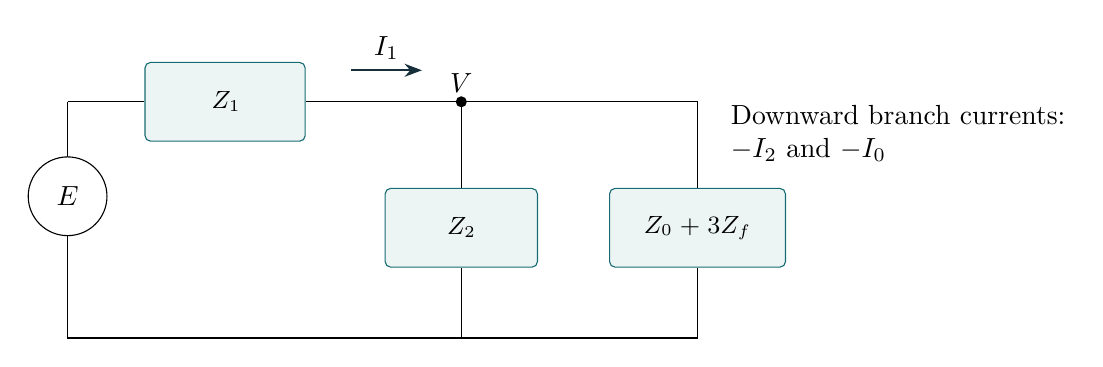
\begin{tikzpicture}
\node[block,text width=1.8cm] (z1) at (2,1.4){$Z_1$};
\draw (0,1.4)--(z1.west);\draw (z1.east)--(5,1.4);\fill (5,1.4)circle(2pt);\node[above] at (5,1.4){$V$};
\draw (0,1.4)--(0,.7);\draw (0,.2)circle(.5);\node at (0,.2){$E$};\draw (0,-.3)--(0,-1.6)--(8,-1.6);
\node[block,text width=1.7cm] (z2) at (5,-.2){$Z_2$};
\node[block,text width=2.0cm] (z0) at (8,-.2){$Z_0+3Z_f$};
\draw (5,1.4)--(z2.north);\draw (z2.south)--(5,-1.6);
\draw (5,1.4)--(8,1.4)--(z0.north);\draw (z0.south)--(8,-1.6);
\draw[arr] (3.6,1.8)--(4.5,1.8)node[midway,above]{$I_1$};
\node[right,align=left] at (8.3,1){Downward branch currents:\\$-I_2$ and $-I_0$};
\end{tikzpicture}
\end{center}
\diagramcaption{LLG equivalent connection, with current-sign convention made explicit. For solid LLG use $Z_f=0$. For LG the three impedances are in series; for LL the zero branch is absent.}

\subsubsection{Solid LLG connection}\slides{Fault, p. 31}
\begin{center}\includegraphics[width=.94\textwidth,height=68mm,keepaspectratio]{Study_Assets/Module3/fault_031.pdf}\end{center}
\diagramcaption{Positive sequence feeds the parallel negative and zero networks. Use the corrected current signs in Section~\ref{faultnumericals}; the diagram does not justify copying the erroneous source arithmetic.}

\subsection{A calculation workflow and powerful checks}
Draw a one-line diagram; state fault type/location and fault impedance definition; select common bases; construct each equipment's sequence connections; reduce to $E,Z_1,Z_2,Z_0$ at the fault; apply boundary conditions; solve sequence currents; transform to phase currents/voltages; convert to actual values at that bus. Finally check
\begin{itemize}
\item LG: $I_b=I_c=0$, $I_a=3I_0$, $V_a=Z_fI_a$.
\item LL: $I_a=0$, $I_b=-I_c$, $I_0=0$, $V_b-V_c=Z_fI_b$.
\item Solid LLG: $I_a=0$, $V_b=V_c=0$, $I_b+I_c=3I_0$.
\item Three phase: equal current magnitudes $120^\circ$ apart, $I_0=I_2=0$.
\end{itemize}
For symmetric short-circuit apparent power, $S_{sc}=\sqrt3V_{LL,\rm nominal}|I_f|$. With $E=1$ p.u., a reactance-only three-phase Thevenin model gives $S_{sc}=S_B/X_{1,\rm pu}$. Nominal voltage is used for this duty convention; the bolted fault-point voltage itself is zero.

\chapterstart{Every class fault calculation, with checks}{faultnumericals}
\subsection{Class case 1: solid three-phase fault, positive impedance 0.20 p.u.}
\slides{Fault-analysis part pp. 19--20}
With $E=1$, $Z_1=\jj0.20$,
\[
 I_1=1/(\jj0.20)=-\jj5=5\angle-90^\circ,\qquad I_0=I_2=0.
\]
\[
 \ans{I_a=5\angle-90^\circ},\quad
 \ans{I_b=5\angle150^\circ},\quad \ans{I_c=5\angle30^\circ}\quad\mathrm{p.u.}
\]
Multiplication by $a^2$ rotates $I_a$ another $-120^\circ$: $-210^\circ$ is the same angle as $150^\circ$. A bare magnitude of 5 does not describe the phase relationships.
\subsection{Class case 2: three-phase current at an 11 kV bus}
\slides{Fault-analysis part pp. 21--22}
$S_B=100$ MVA, $V_B=11$ kV, $Z_1=\jj0.25$ p.u. and $E=1$:
\[
 |I_f|=|1/(\jj0.25)|=4\ \mathrm{p.u.},\quad
 I_B=\frac{100}{\sqrt3(11)}=5.248639\ \mathrm{kA},
\]
\[
 \ans{|I_f|=4(5.248639)=20.9946\ \mathrm{kA}}.
\]
The diagram on the solution slide includes extraneous sequence branches and a different positive label; the question's $Z_1=\jj0.25$ is the value that gives its stated 4 p.u. result. Only the positive network is needed for this balanced fault. Associated short-circuit level is $100/0.25=400$ MVA.
\subsection{Class case 3a: solid LG fault}
\slides{Fault-analysis part pp. 23--24}
Given $Z_1=\jj0.20$, $Z_2=\jj0.20$, $Z_0=\jj0.10$, $E=1$, solid fault on $a$:
\[
 \ans{I_0=I_1=I_2=\frac1{\jj0.50}=-\jj2\ \mathrm{p.u.}},\quad
 \ans{I_a=-\jj6\ \mathrm{p.u.},\quad I_b=I_c=0}.
\]
The sequence voltages are
\[
 V_1=1-(\jj0.2)(-\jj2)=0.6,\quad V_2=-(\jj0.2)(-\jj2)=-0.4,
 \quad V_0=-(\jj0.1)(-\jj2)=-0.2.
\]
Check $V_a=0.6-0.4-0.2=0$. For the same bus, three-phase current is 5 p.u.; this LG current is 6 p.u. Thus a three-phase fault is not always the largest current.
\subsection{Class case 3b: the same LG fault with impedance}
\slides{Fault-analysis part pp. 23, 25}
Now $Z_f=\jj0.05$ p.u.:
\[
 I_0=I_1=I_2=\frac1{\jj(0.2+0.2+0.1+3\times0.05)}
 =-\jj1.538462\ \mathrm{p.u.},
\]
\[
 \ans{I_a=-\jj4.615385\ \mathrm{p.u.},\quad I_b=I_c=0}.
\]
$V_1=0.6923077$, $V_2=-0.3076923$, $V_0=-0.1538462$, so
\[
 V_a=0.2307692=Z_fI_a=(\jj0.05)(-\jj4.615385).
\]
Fault impedance reduces current here. Its factor of three results from the fault phase current being three times each sequence current.
\subsection{Class case 4: LL fault at the receiving end}
\slides{Fault-analysis part pp. 26--29}
All data already share a common p.u. base. Generator $X_{1G}=0.15$, $X_{2G}=0.20$; transformer $X_{1T}=X_{2T}=0.10$; line $X_{1L}=X_{2L}=0.05$. The fault is solid between $b,c$ and $E=1$.
\[
 Z_1=\jj(0.15+0.10+0.05)=\jj0.30,\quad
 Z_2=\jj(0.20+0.10+0.05)=\jj0.35.
\]
\[
 \ans{I_1=-\jj1.538462,\quad I_2=+\jj1.538462,\quad I_0=0}\quad\mathrm{p.u.}
\]
\[
 I_b=-\jj\sqrt3I_1=-2.664694,\qquad I_c=+2.664694,
\]
\[
 \ans{I_a=0,\quad I_b=2.664694\angle180^\circ,\quad I_c=2.664694\angle0^\circ}\quad\mathrm{p.u.}
\]
Check $I_b+I_c=0$. $V_1=1-0.3(1.538462)=0.538462$; $V_2=-(\jj0.35)(+\jj1.538462)=0.538462$. Hence $V_b=V_c=-0.538462$ p.u. under this reference: the faulted phases have equal voltages, not necessarily zero voltage to earth.

\subsection{Class case 5: LLG, with the slide sign error corrected}
\slides{Fault-analysis part pp. 30--33}
$Z_1=\jj0.20$, $Z_2=\jj0.20$, $Z_0=\jj0.10$, $E=1$; solid fault on $b,c$ to earth. The parallel part is
\[
 Z_2\parallel Z_0=\frac{(\jj0.20)(\jj0.10)}{\jj0.30}=\jj0.0666667.
\]
\[
 I_1=\frac1{\jj0.2666667}=-\jj3.75,\qquad
 V=V_1=1-(\jj0.20)(-\jj3.75)=0.25.
\]
From $V_2=-Z_2I_2$ and $V_0=-Z_0I_0$,
\[
 \ans{I_2=-\frac{0.25}{\jj0.20}=+\jj1.25},\qquad
 \ans{I_0=-\frac{0.25}{\jj0.10}=+\jj2.50}\quad\mathrm{p.u.}
\]
Now transform:
\begin{align*}
 I_a&=\jj2.5-\jj3.75+\jj1.25=\ans{0},\\
 I_b&=\jj2.5+a^2(-\jj3.75)+a(\jj1.25)=\ans{-4.330127+\jj3.75},\\
 I_c&=\jj2.5+a(-\jj3.75)+a^2(\jj1.25)=\ans{4.330127+\jj3.75}.
\end{align*}
Thus $|I_b|=|I_c|=5.72822$ p.u. and the earth current is $I_b+I_c=\ans{\jj7.5=3I_0}$ p.u. Also $V_0=V_1=V_2=0.25$, giving $V_b=V_c=0$ and $V_a=0.75$ p.u.
\begin{Caution}{The physical check exposes the arithmetic error}
Slide p. 32 writes $I_2=-0.25/(\jj0.20)$ but evaluates it as $-\jj1.25$. Since $1/\jj=-\jj$, the leading minus makes the result \emph{positive} imaginary. Its $I_0$ has the same error. Slide p. 33 then obtains $I_a=-\jj7.5$, contradicting the stated unfaulted phase-$a$ condition $I_a=0$. The correct 7.5 p.u. value is the magnitude of the total earth current, not current in phase $a$.
\end{Caution}

\subsection{Class case 6: limiting three-phase current with a reactor}
\slides{Fault-analysis part pp. 34--35}
A 20 MVA, 10 kV alternator has $X_d''=5\%=0.05$ p.u. Find additional series reactance to limit a terminal three-phase short circuit to eight times full-load current. Use the machine's ratings as bases and $E=1$.
\[
 I_B=\frac{20}{\sqrt3(10)}=1.154701\ \mathrm{kA},\quad
 I_{\max}=8I_B=9.237604\ \mathrm{kA},\quad
 X_{\rm total,pu}=1/8=0.125.
\]
\[
 \ans{X_{\rm ext,pu}=0.125-0.05=0.075=7.5\%}.
\]
$Z_B=10^2/20=5\ \Omega$, hence $\ans{X_{\rm ext}=0.075(5)=0.375\ \Omega/phase}$. At 50 Hz this corresponds to $L=X/\omega=1.19366$ mH/phase. The current multiple and reactance percentage must use the same machine base; confusing a 5\% reactance with 5 p.u. reverses the scale by a factor of 100.

\chapterstart{Protection: sensing, selectivity and backup}{protection}
\slides{Protection part pp. 1--14, 31, 37}
\subsection{Why protection is needed and what each device does}
Protection reduces the duration and extent of abnormal operation. It cannot prevent every fault. A \textbf{CT} supplies scaled current, a \textbf{VT/PT} supplies scaled voltage, and the \textbf{relay} measures and evaluates them. The relay's trip output energises the breaker trip circuit from a control supply. A latch releases stored spring/pneumatic/hydraulic energy; the \textbf{circuit breaker} separates power contacts and interrupts the current. An alarm can be issued without a trip when the logic requires it.
\begin{center}
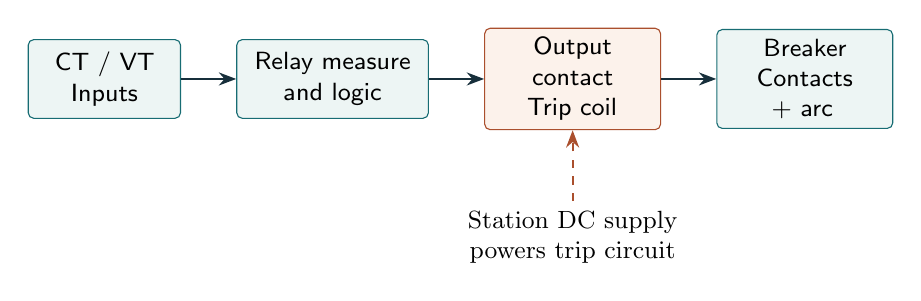
\begin{tikzpicture}[node distance=7mm]
\node[block,text width=1.7cm] (ct){CT / VT\\Inputs};
\node[block,text width=2.2cm,right=of ct] (l){Relay measure\\and logic};
\node[hot,text width=2.0cm,right=of l] (t){Output contact\\Trip coil};
\node[block,text width=2.0cm,right=of t] (b){Breaker\\Contacts + arc};
\draw[arr] (ct)--(l);\draw[arr] (l)--(t);\draw[arr] (t)--(b);
\node[below=9mm of t,align=center,font=\small] (dc){Station DC supply\\powers trip circuit};\draw[control] (dc)--(t);
\end{tikzpicture}
\end{center}
Total clearing time includes measurement/relay decision, any intentional delay, output/auxiliary operation, breaker opening and arcing to final current interruption. ``Instantaneous relay'' means no intentional time delay; it still has finite operating time. The relay does not directly switch thousands of amperes through its small output contacts.

\subsubsection{Relay and breaker recognition}\slides{Protection, p. 5}
\begin{center}\includegraphics[width=.94\textwidth,height=68mm,keepaspectratio]{Study_Assets/Module3/pr_005.pdf}\end{center}
\diagramcaption{The relay decides; the breaker interrupts the power circuit. They have different current ratings and functions.}

\subsubsection{CT-relay-trip-coil circuit}\slides{Protection, p. 16}
\begin{center}\includegraphics[width=.94\textwidth,height=68mm,keepaspectratio]{Study_Assets/Module3/pr_016.pdf}\end{center}
\diagramcaption{Follow the low-power sensing circuit separately from the DC trip supply. A relay contact energizes the breaker trip coil.}

\subsection{Requirements and their tradeoffs}
\begin{center}\small
\begin{tabularx}{\textwidth}{L{.23\textwidth}Y}
\toprule Requirement & Meaning and useful test\\\midrule
Selectivity & Isolate the faulted section while keeping healthy supply where possible. A fault near one feeder end should not unnecessarily trip the whole substation.\\
Speed & Clear quickly enough to limit damage and preserve stability. Some deliberate delay is needed for graded backup.\\
Sensitivity & Detect the minimum credible fault, including weak-source/far-end conditions. Pickup still must avoid permissible load and transients.\\
Stability/security & Avoid unwanted operation for external faults, allowable load, CT error, inrush or other non-trip conditions relevant to the scheme.\\
Dependability & Operate for faults the scheme is assigned to clear. Reliability includes both dependable operation and security against false trips.\\
Simplicity/economy & Use a maintainable, testable arrangement suited to the protected equipment and required reliability.\\\bottomrule
\end{tabularx}\end{center}
The slides emphasise four S's: selectivity, stability, speed and sensitivity. They must be interpreted within a declared protection zone; a backup relay \emph{is intended} to clear a fault outside its primary zone if primary protection fails.
\subsection{Primary protection, local backup and remote backup}
\textbf{Primary/main protection} is assigned to clear faults in its protected zone with the intended speed/selectivity. It can include intentional delay; ``primary'' is a responsibility, not a guarantee of instantaneous action. \textbf{Backup protection} acts if a main relay, trip circuit, DC supply, communications path or breaker fails. It normally waits long enough to allow the primary scheme to work.

Local backup may be an independent relay system or breaker-failure scheme at the same station. Remote backup is provided by relays/breakers at another station; it can cover local failure but may remove more healthy equipment and may be less sensitive because of network infeed. Independent main schemes can be used to reduce common failure modes.

\subsubsection{Primary and backup arrangement}\slides{Protection, p. 6}
\begin{center}\includegraphics[width=.94\textwidth,height=68mm,keepaspectratio]{Study_Assets/Module3/pr_006.pdf}\end{center}
\diagramcaption{The feeder device isolates its local fault first. The upstream device supplies delayed backup; settings depend on the actual installation.}

Zones are associated with equipment such as generators, transformers, buses and lines. CT locations define many unit-protection boundaries. Adjacent zones overlap around breakers so a fault at a boundary can be cleared. This equipment-zone overlap is different from the numbered reach zones of one distance relay.
\begin{center}
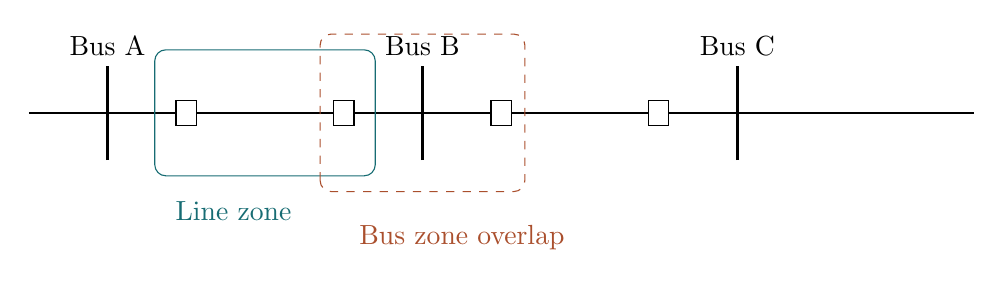
\begin{tikzpicture}
\draw[thick] (0,0)--(12,0);
\foreach \x/\t in {1/A,5/B,9/C}{\draw[very thick] (\x,-.6)--(\x,.6);\node[above] at (\x,.6){Bus \t};}
\foreach \x in {2,4,6,8}{\draw[fill=white] (\x-.13,-.16)rectangle(\x+.13,.16);}
\draw[teal,rounded corners] (1.6,-.8)rectangle(4.4,.8);
\draw[rust,dashed,rounded corners] (3.7,-1)rectangle(6.3,1);
\node[below,teal] at (2.6,-1){Line zone};\node[below,rust] at (5.5,-1.3){Bus zone overlap};
\end{tikzpicture}
\end{center}
\diagramcaption{Conceptual overlapping protection boundaries. Practical CT placements, breaker-failure logic and zone assignments must be specified for an actual station.}

\subsubsection{Overlapping protection zones}\slides{Protection, p. 31}
\begin{center}\includegraphics[width=.94\textwidth,height=68mm,keepaspectratio]{Study_Assets/Module3/pr_031.pdf}\end{center}
\diagramcaption{CT locations define zone boundaries around breakers. This equipment-zone sketch is distinct from distance-relay reach zones.}

\subsection{Relay coordination by time and current}
In a radial feeder, all upstream relays can see a downstream fault. \textbf{Time grading} sets the nearest downstream relay to trip first; successive upstream relays provide delayed backup. Definite-time grading is simple but can make source-end fault clearing slow. Inverse-time curves permit shorter times for higher current, yet coordination must be checked across the credible fault-current range.

\textbf{Current grading} uses decreasing available fault current with distance in a simple radial network. Choose pickup above maximum permissible load and below the minimum fault current that the relay must detect, with required margins. Similar fault magnitudes at adjacent positions, multiple sources and changing topology limit pure current discrimination. Time-current grading combines pickup and delay settings.

\subsubsection{Time grading}\slides{Protection, p. 10}
\begin{center}\includegraphics[width=.94\textwidth,height=68mm,keepaspectratio]{Study_Assets/Module3/pr_010.pdf}\end{center}
\diagramcaption{The source illustration gives example delays. Coordination needs a margin covering breaker time, relay error and overtravel, not these exact universal settings.}

\subsubsection{Current grading}\slides{Protection, p. 11}
\begin{center}\includegraphics[width=.94\textwidth,height=68mm,keepaspectratio]{Study_Assets/Module3/pr_011.pdf}\end{center}
\diagramcaption{Compare pickup and fault current along a radial feeder. Current grading alone fails where adjacent fault currents are too similar.}
\begin{Worked}{Additional example: a concrete coordination margin}
For one downstream fault, downstream relay operating time is 0.20 s and its breaker interruption time after trip output is 0.06 s. If the specified allowance for overshoot/tolerances is 0.10 s, upstream relay operating time must be at least $0.20+0.06+0.10=0.36$ s under this simplified coordination rule. This is a 0.16 s difference between relay times, not a universal setting. Repeat at relevant fault locations/current levels.
\end{Worked}

\Needspace{115mm}
\subsection{Breaker failure and interpreting slide timing values}
Breaker-failure logic starts after a valid trip initiation and checks whether current and/or breaker status indicates failure to interrupt. A timed failure output can retrip or trip adjacent/upstream breakers to remove every source feeding the fault. Reset criteria avoid wider tripping after successful clearance. A breaker auxiliary contact alone and current alone each have limitations; actual schemes specify their supervision.

The slides give illustrative values: 3--10 cycles for a fault-clearing chain, 15--17 cycles for a breaker-failure timer, 0.2--0.5 s coordination intervals, and a 0.4 s electromechanical coordination example. They are not universal rules. At \textbf{50 Hz}, one cycle is 20 ms: 0.4 s is \textbf{20 cycles}, not the 24 cycles printed in the slides (24 cycles corresponds to 60 Hz). CT error/saturation is not automatically a separate fixed 12-cycle delay that is added to every fault. Specify the actual relay, breaker, tolerances and coordination assumptions.

\subsection{Equipment applications and context from the slides}
Transformer and generator differential protection are typical unit schemes. Transformer overcurrent can provide backup; a Buchholz gas/oil-motion relay applies to appropriate oil-filled conservator arrangements and detects particular internal abnormalities, so it is not a generic backup substitute for every transformer fault. Generator protection may include negative sequence, reverse power, loss of excitation and stator earth-fault functions. Lines may use distance, directional OC, line differential or communication-assisted schemes depending on their application.

Numerical IEDs can combine protection, metering, recording, control and communication. The slides' claims of 99.99\% availability or immunity to network changes are aspirations/overstatements, not guarantees from selecting four relay principles. Adaptive settings and data-based fault detection are contextual developments; dependable, tested protection and secure configuration remain essential.

\chapterstart{The four protection principles}{principles}
\slides{Protection part pp. 13--38}
\subsection{Overcurrent: magnitude plus a timing rule}
An OC element picks up when measured current exceeds $I_{pickup}$. It may operate with no intentional delay (instantaneous, device 50), after a preset delay (definite time), or after a current-dependent delay (inverse-time, commonly device 51). A high-set instantaneous element supplements a delayed element when its reach can be made selective.

Define current multiple / plug-setting multiplier (PSM):
\[
 M=\frac{I_{\rm measured,secondary}}{I_{\rm pickup,secondary}}
 =\frac{I_{\rm primary}}{I_{\rm primary,pickup}}.
\]
CT ratio and pickup must be applied consistently. A 400/5 A CT has ratio 80. Pickup 5 A secondary means 400 A primary; a 2000 A primary fault gives 25 A secondary and $M=5$. ``Pickup 100\%'' depends on the relay's nominal-current base; it is not 100\% of fault current.

One widely used standard-inverse educational curve is
\[
 \ans{t=\mathrm{TMS}\frac{0.14}{M^{0.02}-1}},\qquad M>1.
\]
Other inverse shapes use different coefficients/exponents (for example very inverse $13.5/(M-1)$ and extremely inverse $80/(M^2-1)$, with the appropriate time multiplier). Manufacturer implementations and reset logic must be specified; one time-dial number is not interchangeable between all relay families. The curve defines relay operating time, not total breaker clearing time. The coefficients are cross-checked against the linked SEL technical manual in the references.
\begin{center}
\begin{tikzpicture}[x=.62cm,y=.85cm]
\draw[arr] (0,0)--(12,0)node[right]{$M$};\draw[arr] (0,0)--(0,5)node[above]{$t$};
\draw[teal,thick] plot[smooth] coordinates{(1.1,4.5)(1.5,3.1)(2,2.2)(3,1.5)(5,.95)(8,.65)(11,.5)};
\draw[rust,thick,dashed] (1,2)--(11,2)node[right]{Definite time};
\node[teal,above] at (6,1.1){Inverse};\draw[gray,dotted] (1,0)--(1,4.5);\node[below] at (1,0){1};
\end{tikzpicture}\end{center}
\diagramcaption{Conceptual time-current characteristics, not a calibrated manufacturer curve. Below pickup the element does not trip under this basic rule.}

\subsubsection{Overcurrent characteristic family}\slides{Protection, p. 17}
\begin{center}\includegraphics[width=.94\textwidth,height=68mm,keepaspectratio]{Study_Assets/Module3/pr_017.pdf}\end{center}
\diagramcaption{Definite time, inverse, very inverse and extremely inverse curves describe operating time versus current multiple. Instantaneous still has finite operating time.}
\begin{Worked}{Additional example: current multiple and inverse time}
For the 400/5 A CT above, choose 5 A secondary pickup and TMS $=0.1$. At 2000 A primary, $M=5$ and $t=0.1(0.14)/(5^{0.02}-1)=0.427972$ s. At 4000 A, $M=10$ gives $t=0.297060$ s. Higher current gives shorter relay time. Add the relevant output/breaker delays to estimate total clearing time.
\end{Worked}
OC is well suited to many radial feeders. It does not directly identify direction or compare boundary currents. Weak-source far-end faults and significant distributed generation can complicate magnitude-based selectivity.

\subsection{Directional: determine which way a fault lies}
A directional element compares current phase with a \emph{polarising/reference} voltage or another suitable reference. It distinguishes forward and reverse relative to the installed CT/VT polarity and chosen relay characteristic. There is no universal rule that every fault reverses normal power flow. A relay may deliberately trip for \emph{forward} faults while blocking reverse faults.

For an elementary voltage-current induction model, operating torque may be written
\[
 T_{op}=K|V||I|\cos(\theta-\tau)-T_{restraint},
\]
where $\theta=\angle V-\angle I$ under the declared convention and $\tau$ is the maximum-torque/characteristic angle. The actual sign convention is relay specific. Directional OC combines directional permission with current pickup/timing:
\[
 \text{Trip}=(\text{forward permission})\ \mathrm{AND}\ (\text{OC condition/timer complete}).
\]
A directional element is therefore not simply an ammeter and not necessarily a complete fault detector on its own. Polarising voltage can be weak for a close-in fault; suitable cross/memory/sequence polarisation helps practical implementations.
\begin{center}
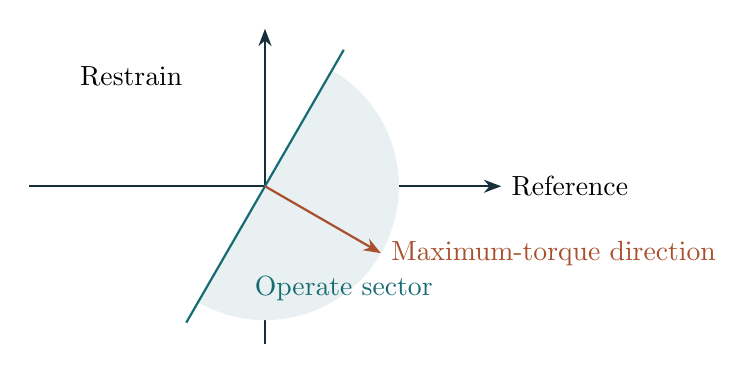
\begin{tikzpicture}
\draw[arr] (-3,0)--(3,0)node[right]{Reference};\draw[arr] (0,-2)--(0,2);
\fill[teal!10] (0,0)--(60:1.7)arc(60:-120:1.7)--cycle;
\draw[teal,thick] (-120:2)--(60:2);\draw[arr,rust] (0,0)--(-30:1.7)node[right]{Maximum-torque direction};
\node[teal] at (1,-1.3){Operate sector};\node at (-1.7,1.4){Restrain};
\end{tikzpicture}\end{center}
\diagramcaption{Illustrative half-plane directional characteristic. Axes and angle reference must match the relay's voltage/current convention; the sector shown is not a universal setting.}

\subsubsection{Current and voltage coils}\slides{Protection, p. 18}
\begin{center}\includegraphics[width=.94\textwidth,height=68mm,keepaspectratio]{Study_Assets/Module3/pr_018.pdf}\end{center}
\diagramcaption{A directional element combines current and a polarizing quantity. An ordinary nondirectional overcurrent element need not have a voltage coil.}

\subsubsection{Forward and reverse fault phasors}\slides{Protection, p. 24}
\begin{center}\includegraphics[width=.94\textwidth,height=68mm,keepaspectratio]{Study_Assets/Module3/pr_024.pdf}\end{center}
\diagramcaption{Direction depends on the polarizing-voltage/current relationship and relay characteristic angle, not current magnitude alone.}

\subsubsection{Directional induction construction}\slides{Protection, p. 25}
\begin{center}\includegraphics[width=.94\textwidth,height=68mm,keepaspectratio]{Study_Assets/Module3/pr_025.pdf}\end{center}
\diagramcaption{Identify potential coil, current coil, moving disc and trip contacts. The configured torque direction defines forward operation; source prose must not be read as a universal reversed convention.}

\subsection{Distance: impedance as electrical reach}
A distance element estimates \emph{apparent impedance} from an appropriate voltage/current fault loop. For a simple fault on a uniform line, the measured loop impedance relates to impedance per length and distance to the fault. A low apparent impedance inside a selected characteristic can indicate a fault within reach.

For a phase-$b$-$c$ loop,
\[
 Z_{bc,app}=\frac{V_b-V_c}{I_b-I_c}.
\]
For a compensated phase-$a$ earth loop, one common convention is
\[
 Z_{aG,app}=\frac{V_a}{I_a+k_0(3I_0)},\qquad
 k_0=\frac{Z_{0,line}-Z_{1,line}}{3Z_{1,line}}.
\]
Some relay texts absorb the factor three into a coefficient multiplying $I_0$ instead. Always match the current and coefficient definitions. This supplement shows why one bare $V_a/I_a$ formula is not sufficient for every fault type.

Elementary characteristics in the $R$-$X$ plane include \textbf{impedance} (circle centred at the origin), \textbf{reactance} (a reach boundary in reactance, requiring suitable directional/control logic) and \textbf{mho} (a circle through the origin along the characteristic angle, providing directional behaviour in its ideal form).
\begin{center}
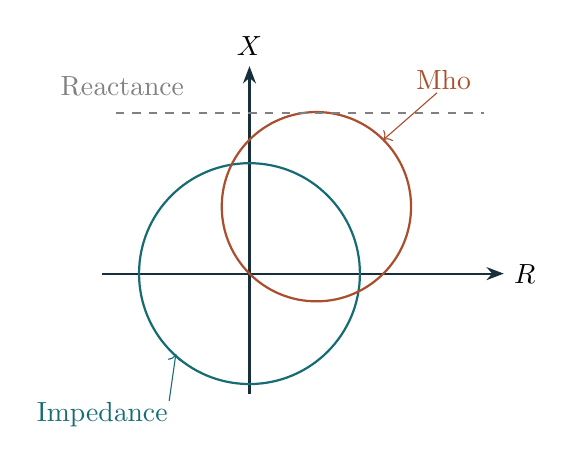
\begin{tikzpicture}[scale=.85]
\draw[arr] (-2.2,0)--(3.8,0)node[right]{$R$};\draw[arr] (0,-1.8)--(0,3.1)node[above]{$X$};
\draw[teal,thick] (0,0)circle(1.65);\draw[rust,thick] (1,1)circle(1.4142);
\draw[gray,dashed] (-2,2.4)--(3.5,2.4);
\node[teal] at (-2.2,-2.1){Impedance};\node[rust] at (2.9,2.9){Mho};\node[gray] at (-1.9,2.8){Reactance};
\draw[teal,->] (-1.2,-1.9)--(-1.1,-1.2);\draw[rust,->] (2.8,2.7)--(2,2);
\end{tikzpicture}\end{center}
\diagramcaption{Separate ideal characteristic sketches superposed for comparison. Reach and polarisation in an actual relay require the specified implementation.}

\textbf{Zone 1} commonly underreaches the protected line and has no intentional delay. \textbf{Zone 2} extends beyond the remote end with a delay. \textbf{Zone 3} gives further delayed backup where required. The slides use 80\%, 120\%, approximately 0.35 s and 0.8 s as examples; they are not mandatory settings for every line. Reach must account for adjacent lines, measurement error, infeed and coordination.

Distance protection is less dependent on fault-current magnitude than simple OC, but it is not independent of all loading/source conditions. Fault resistance, remote infeed, power swings, load encroachment, CT/VT error and incorrect line data can change apparent impedance or the decision. A low $|V/I|$ must be assessed within its characteristic and supervision.

\subsubsection{Distance sensing and processing}\slides{Protection, p. 28}
\begin{center}\includegraphics[width=.94\textwidth,height=68mm,keepaspectratio]{Study_Assets/Module3/pr_028.pdf}\end{center}
\diagramcaption{The selected voltage/current loop estimates apparent impedance. Fault resistance, infeed and instrument errors affect the estimate.}

\subsubsection{Distance reaches}\slides{Protection, p. 30}
\begin{center}\includegraphics[width=.94\textwidth,height=68mm,keepaspectratio]{Study_Assets/Module3/pr_030.pdf}\end{center}
\diagramcaption{The class 80/120 percent settings and delays are illustrative. Zone reaches must coordinate with neighbouring lines.}
\begin{Worked}{Additional example: reach conversion to relay ohms}
A line has $Z_L=10+\jj40\ \Omega$ primary. An 80\% reach is $8+\jj32\ \Omega$. CT ratio is 400/5 $=80$, VT ratio is 110000/110 $=1000$. Because $V_s=V_p/1000$ and $I_s=I_p/80$, relay impedance is $Z_s=Z_p(80/1000)$. Reach is therefore $0.64+\jj2.56\ \Omega$ secondary. Interchanging the CT and VT ratios would give a severe reach error.
\end{Worked}

\subsection{Differential: compare the zone's boundary currents}
Apply KCL to currents crossing the protected equipment boundary. After CT ratio, polarity and any required transformer phase-shift compensation, external load/fault current ideally balances; an internal fault creates a nonzero sum.

With $I_1$ defined into a two-terminal zone and $I_2$ defined out of it,
\[
 I_{diff}=|I_1-I_2|,\qquad I_{bias}=\frac{|I_1|+|I_2|}{2}.
\]
Alternatively define every current into the zone and use their algebraic sum. Do not mix these conventions. A simplified biased rule is
\[
 I_{diff}>I_{min}+sI_{bias},
\]
where $s$ is the restraint slope. Some devices instead use a maximum of pickup and slope thresholds, multiple slopes or another bias definition; specify the characteristic used.
\begin{center}
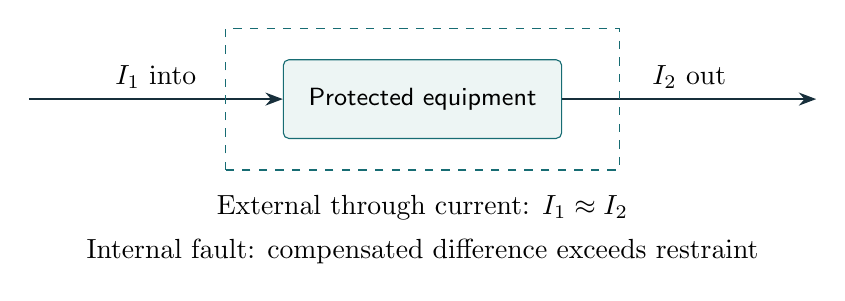
\begin{tikzpicture}
\node[block,text width=3.3cm] (e) at (5,0){Protected equipment};
\draw[arr] (0,0)--(e.west)node[midway,above]{$I_1$ into};
\draw[arr] (e.east)--(10,0)node[midway,above]{$I_2$ out};
\draw[teal,dashed] (2.5,-.9)rectangle(7.5,.9);
\node[below] at (5,-1.1){External through current: $I_1\approx I_2$};
\node[below] at (5,-1.65){Internal fault: compensated difference exceeds restraint};
\end{tikzpicture}\end{center}
CT mismatch and saturation can create spill current during an external fault. Bias improves security while retaining internal-fault sensitivity. Transformer differential additionally needs ratio/vector-group compensation and suitable inrush/overexcitation restraint or blocking. Line differential may need communications and charging-current consideration. No scheme is automatically immune to every external condition.

\subsubsection{Differential balance and internal fault}\slides{Protection, p. 34}
\begin{center}\includegraphics[width=.94\textwidth,height=68mm,keepaspectratio]{Study_Assets/Module3/pr_034.pdf}\end{center}
\diagramcaption{With all currents referenced into the zone, their sum is approximately zero for through current and nonzero for an internal fault.}

\subsubsection{Pilot-wire differential circuit}\slides{Protection, p. 35}
\begin{center}\includegraphics[width=.94\textwidth,height=68mm,keepaspectratio]{Study_Assets/Module3/pr_035.pdf}\end{center}
\diagramcaption{Trace CT secondary circulation during an external fault. Ideally no spill current flows through the operating coil.}
\begin{Worked}{Additional example: why bias is useful}
Use the simplified rule with $I_{min}=0.2$ A and $s=0.30$. Measured compensated through currents $I_1=10$, $I_2=9.5$ A give $I_{diff}=0.5$ A, $I_{bias}=9.75$ A, threshold $3.125$ A: restrained. For $I_1=6$, $I_2=1$ A, the difference is 5 A, bias 3.5 A, threshold 1.25 A: operates. These are educational values for the specified characteristic, not actual protection settings.
\end{Worked}

\subsection{Compare the four principles}
\begin{center}\small
\begin{tabularx}{\textwidth}{L{.16\textwidth}L{.24\textwidth}L{.24\textwidth}Y}
\toprule Principle & Main quantity & Typical use & Main limitation to remember\\\midrule
OC & Current magnitude and time & Radial feeders, backup & No inherent direction/location; coordination changes with fault level.\\
Directional & Angle relation / directional torque & Multi-source feeders, directional OC & Reference/polarity and polarisation matter.\\
Distance & Fault-loop apparent impedance & Transmission-line reach zones & Fault resistance, infeed, load/swing and measurement can affect reach.\\
Differential & Compensated current balance & Transformer, generator, bus, line & CT errors/saturation, compensation and communication where used.\\\bottomrule
\end{tabularx}\end{center}

\chapterstart{Induction-type electromechanical relays}{induction}
\slides{Protection part pp. 18, 39--57}
The syllabus limits detailed electromechanical study to \emph{induction type}. Attraction/solenoid relays appear in the slides as context and as instantaneous elements; their separate construction derivations are not needed here. Induction operation requires alternating flux and therefore does not operate from steady DC by the same principle.

\subsubsection{Electromagnetic relay gallery}\slides{Protection, p. 42}
\begin{center}\includegraphics[width=.94\textwidth,height=68mm,keepaspectratio]{Study_Assets/Module3/pr_042.pdf}\end{center}
\diagramcaption{These photographs provide recognition context. Attraction and induction are different mechanisms; the syllabus develops induction type.}
\subsection{Two fluxes and an aluminium moving element}
Two alternating magnetic fluxes are displaced in \emph{space} and \emph{time}. Each induces eddy currents in a conducting nonmagnetic disc/cup. Interaction between one flux and currents induced by the other produces average torque. With sinusoidal fluxes
\[
 \phi_1=\Phi_1\sin\omega t,\qquad \phi_2=\Phi_2\sin(\omega t+\delta),
\]
induced currents depend on flux rate of change. The net average cross-interaction is proportional to
\[
 \ans{T_{op}=K\Phi_1\Phi_2\sin\delta}.
\]
If either flux is absent, or their phase displacement is zero, ideal net driving torque vanishes. For an OC construction with both fluxes proportional to the same relay current and approximately fixed phase displacement,
\[
 T_{net}\approx K_1I^2-K_2,
\]
where $K_2$ represents spring/restraint torque in the simple model. Pickup occurs when driving torque exceeds restraint. A permanent magnet produces eddy-current braking approximately proportional to disc speed; bearings/friction and magnetic saturation modify the real curve.

It is \emph{operating torque} that follows the approximate $I^2$ dependence. Disc speed is not universally proportional to $I$ or exactly $I^2$: net torque, braking, saturation and acceleration matter. This corrects the inconsistent shorthand in the slide summaries.
\begin{center}
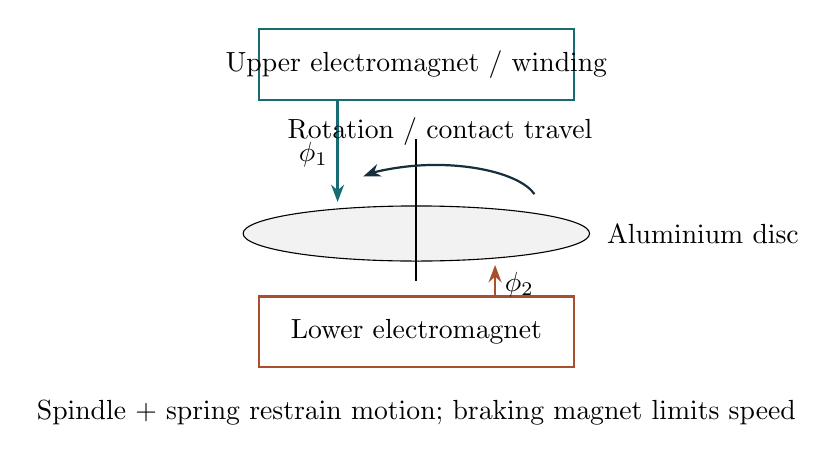
\begin{tikzpicture}
\draw[teal,thick] (0,1.7)rectangle(4,2.6);\node at (2,2.15){Upper electromagnet / winding};
\draw[rust,thick] (0,-1.7)rectangle(4,-.8);\node at (2,-1.25){Lower electromagnet};
\draw[fill=gray!10] (2,0)ellipse(2.2 and .35);\draw[thick] (2,-.6)--(2,1.2);
\node[right] at (4.3,0){Aluminium disc};
\draw[arr,teal] (1,1.7)--(1,.4);\draw[arr,rust] (3,-.8)--(3,-.4);
\node[left] at (1,1){$\phi_1$};\node[right] at (3,-.65){$\phi_2$};
\draw[arr] (3.5,.5)arc(15:135:1.3 and .5);\node[above] at (2.3,1){Rotation / contact travel};
\node[below,align=center] at (2,-2){Spindle + spring restrain motion; braking magnet limits speed};
\end{tikzpicture}\end{center}
\diagramcaption{Functional disc-relay sketch. Spatially displaced flux paths act on the disc; the sketch omits detailed iron-core and tap geometry.}

\subsubsection{Double-winding induction-disc construction}\slides{Protection, p. 44}
\begin{center}\includegraphics[width=.94\textwidth,height=68mm,keepaspectratio]{Study_Assets/Module3/pr_044.pdf}\end{center}
\diagramcaption{Identify the two electromagnets, aluminium disc, spindle, spring, moving/fixed contacts and auxiliary winding connections.}

\subsection{Three ways to obtain the phase-displaced flux}
\textbf{Shaded pole:} a copper shading ring surrounds part of a magnetic pole. Alternating main flux induces current in this ring, whose opposing field delays the shaded flux relative to the unshaded part. Both flux regions act on the disc to produce torque. The phase delay depends on the design; the slide's 40--50$^\circ$ is illustrative, not an invariant.

\textbf{Watt-hour-meter / double-winding structure:} an upper E-shaped magnet carries primary and secondary windings; an induced secondary current energises a lower U-shaped magnet. Circuit resistance/inductance produces a phase displacement between upper and lower fluxes. A tapped primary winding provides current-setting adjustment. Closing the designed secondary circuit enables its second flux and torque; opening that internal control path prevents the ideal driving torque. This is a description of the relay's magnetic circuit, not a suggestion to open an energised external CT secondary.

\textbf{Induction cup:} a light conducting cup rotates around a stationary iron core between two or more electromagnets. Phase-displaced fluxes create a rotating field and induced cup currents. Low inertia and high torque-to-inertia ratio permit fast response; it is used in suitable directional/distance constructions. The slide's approximately 0.01 s is an example, not every cup relay's operating time.
\begin{center}\small
\begin{tabularx}{\textwidth}{L{.22\textwidth}L{.35\textwidth}Y}
\toprule Structure & Source of displacement & Recognition point\\\midrule
Shaded pole & Shading-ring induced current & One pole face split into shaded/unshaded regions.\\
Double winding & Induced secondary and differing magnetic/electrical paths & Upper/lower magnets with disc between them.\\
Cup & Multiple phase-displaced coil fluxes & Light cup around fixed central core.\\\bottomrule
\end{tabularx}\end{center}

\subsubsection{Shaded-pole induction structure}\slides{Protection, p. 47}
\begin{center}\includegraphics[width=.94\textwidth,height=68mm,keepaspectratio]{Study_Assets/Module3/pr_047.pdf}\end{center}
\diagramcaption{The copper shading ring delays one portion of the pole flux. Spatially and temporally displaced fluxes produce disc torque.}

\subsubsection{Watt-hour-meter induction structure}\slides{Protection, p. 50}
\begin{center}\includegraphics[width=.94\textwidth,height=68mm,keepaspectratio]{Study_Assets/Module3/pr_050.pdf}\end{center}
\diagramcaption{The winding arrangement produces two phase-displaced fluxes through the disc. The permanent magnet supplies braking torque.}

\subsubsection{Induction-cup construction}\slides{Protection, p. 53}
\begin{center}\includegraphics[width=.94\textwidth,height=68mm,keepaspectratio]{Study_Assets/Module3/pr_053.pdf}\end{center}
\diagramcaption{The light conducting cup rotates in the air gap around a stationary iron core. Multiple poles create the required flux interaction.}

\subsection{Pickup, time dial and inverse timing}
\textbf{Current tap / plug setting} adjusts pickup. \textbf{Time dial} changes required disc travel/contact angle and thereby operating time at a stated current multiple. A larger travel generally delays operation. The curve shape is determined largely by the relay construction; moving a time dial does not turn every fixed mechanical curve into any desired curve.

Above pickup, higher current generally gives larger net torque and shorter time to travel to the contact. Magnetic saturation and design produce the chosen inverse/IDMT characteristic. ``Inverse definite minimum time'' means the curve approaches a minimum-time region; it does not mean delay is exactly $1/I$ at every current. After current falls, the spring returns the disc and contacts reset, with possible time/overshoot effects that matter in coordination.

Traditional separate phase elements were common, but the slide's requirement of a minimum three relay units is not universal: some three-phase three-wire OC arrangements can use two phase elements with appropriate ground protection. Describe the required protection coverage rather than assuming one specific device count.
\checkq{Why do two equal, in-phase fluxes fail to produce ideal induction torque?}{$\sin\delta=0$ when their phase displacement is zero. The cross interactions cancel on average. The moving element needs both spatial and time displacement of the AC fluxes.}

\chapterstart{Static, microprocessor and numerical relays}{digital}
\slides{Protection part pp. 12, 58--74}
\subsection{Static relays: the decision is electronic}
Static relays use analogue electronic measuring/comparing circuits rather than a moving disc for the decision. They can still have electromechanical output contacts; ``static'' does not imply every part of the trip chain has no movement. Auxiliary power supplies, transducer isolation, component drift and surge immunity are relevant.
\subsubsection{Static time-overcurrent block diagram}
\begin{center}
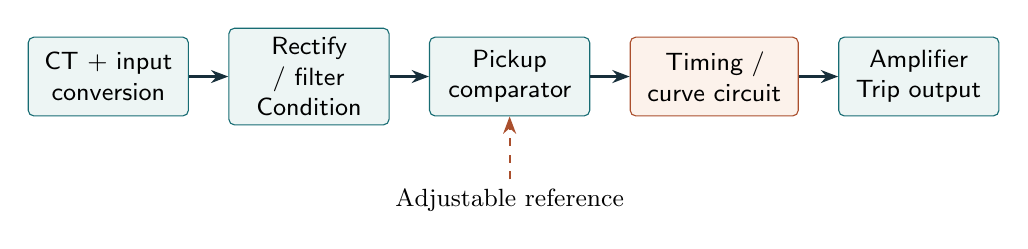
\begin{tikzpicture}[node distance=5mm]
\node[block,text width=1.8cm] (ct){CT + input\\conversion};
\node[block,text width=1.8cm,right=of ct] (rect){Rectify / filter\\Condition};
\node[block,text width=1.8cm,right=of rect] (comp){Pickup\\comparator};
\node[hot,text width=1.9cm,right=of comp] (timer){Timing /\\curve circuit};
\node[block,text width=1.8cm,right=of timer] (out){Amplifier\\Trip output};
\foreach \a/\b in {ct/rect,rect/comp,comp/timer,timer/out}{\draw[arr] (\a)--(\b);}
\node[below=8mm of comp,font=\small] (ref){Adjustable reference};\draw[control] (ref)--(comp);
\end{tikzpicture}\end{center}
The CT-derived signal is converted to a usable voltage and rectified/filtered or otherwise conditioned. A comparator recognises pickup. A timing circuit, such as an RC charging arrangement with current-dependent charging/threshold control, implements the required delay. An amplifier/output device energises the trip stage. Functional ordering can differ: the class diagram places a level comparator after the timing stage. Either drawing must explain where current pickup and timer-completion decisions occur. Auxiliary DC supply supports the electronic and output circuits.
\subsubsection{Static instantaneous overcurrent block diagram}
\begin{center}
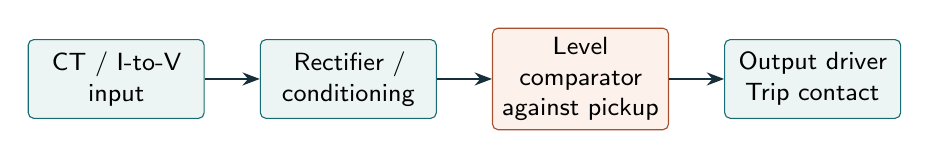
\begin{tikzpicture}[node distance=7mm]
\node[block,text width=2cm] (ct){CT / I-to-V\\input};
\node[block,text width=2cm,right=of ct] (re){Rectifier /\\conditioning};
\node[hot,text width=2cm,right=of re] (co){Level comparator\\against pickup};
\node[block,text width=2cm,right=of co] (ou){Output driver\\Trip contact};
\draw[arr] (ct)--(re);\draw[arr] (re)--(co);\draw[arr] (co)--(ou);
\end{tikzpicture}\end{center}
There is no intentional timing network in the 50 path. Filtering, comparator response and output contacts still take time. The slide's 8--16 ms is an illustrative operating range, not the definition of instantaneous. If directional supervision is added, a VT path and phase comparator supply permission to the OC output/timer; this covers the directional static diagram in the source.

\subsubsection{Static device gallery}\slides{Protection, p. 59}
\begin{center}\includegraphics[width=.94\textwidth,height=68mm,keepaspectratio]{Study_Assets/Module3/pr_059.pdf}\end{center}
\diagramcaption{Electronic measuring circuits replace the moving measuring element. The output may still use an electromechanical auxiliary contact.}

\subsubsection{Static and directional static blocks}\slides{Protection, p. 61}
\begin{center}\includegraphics[width=.94\textwidth,height=68mm,keepaspectratio]{Study_Assets/Module3/pr_061.pdf}\end{center}
\diagramcaption{The first diagram shows rectifier, measuring circuit, amplifier, output and trip supply. The second includes phase comparison for direction. Compare the clearly separated time-overcurrent and instantaneous diagrams in Section~\ref{digital}.}

\subsubsection{Instantaneous static chain}\slides{Protection, p. 62}
\begin{center}\includegraphics[width=.94\textwidth,height=68mm,keepaspectratio]{Study_Assets/Module3/pr_062.pdf}\end{center}
\diagramcaption{Rectification/conditioning, comparison and output trigger replace the induction delay. A comparator reference determines pickup.}

\subsection{Microprocessor relay: sampling and a programmed decision}
A hardware architecture includes CT/VT input conversion/isolation, signal conditioning, anti-alias filtering, sample-and-hold where required, analogue multiplexer for multiple channels if used, ADC, processor, memory, clock, digital inputs, output drivers and an auxiliary supply.
\begin{center}
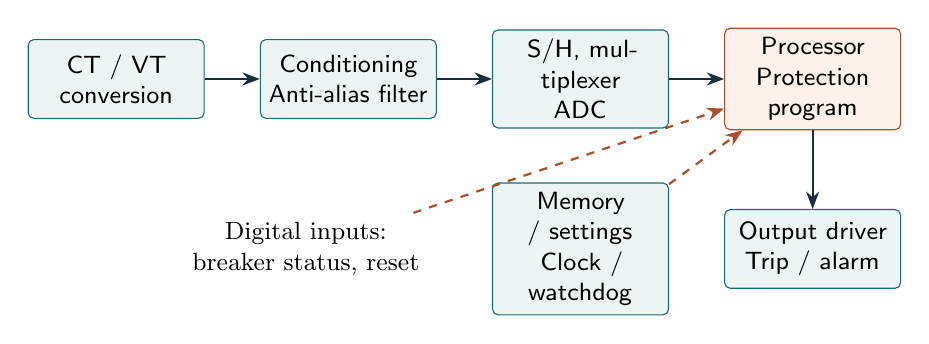
\begin{tikzpicture}[node distance=7mm]
\node[block,text width=2cm] (in){CT / VT\\conversion};
\node[block,text width=2cm,right=of in] (fi){Conditioning\\Anti-alias filter};
\node[block,text width=2cm,right=of fi] (ad){S/H, multiplexer\\ADC};
\node[hot,text width=2cm,right=of ad] (cpu){Processor\\Protection program};
\draw[arr] (in)--(fi);\draw[arr] (fi)--(ad);\draw[arr] (ad)--(cpu);
\node[block,text width=2cm,below=10mm of cpu] (ou){Output driver\\Trip / alarm};\draw[arr] (cpu)--(ou);
\node[block,text width=2cm,left=of ou] (me){Memory / settings\\Clock / watchdog};\draw[control] (me)--(cpu);
\node[left=8mm of me,align=center,font=\small] (di){Digital inputs:\\breaker status, reset};\draw[control] (di)--(cpu);
\end{tikzpicture}\end{center}
The class's older CT $\to$ I/V $\to$ rectifier $\to$ multiplexer $\to$ ADC $\to$ 8085 arrangement is a particular magnitude-based implementation. A modern waveform-sampling numerical relay can digitise conditioned AC directly; a rectifier is not mandatory before every ADC. ADC, multiplexer and processor ports handle measurement/control data, not power-line fault current.

\subsubsection{Digital relay recognition}\slides{Protection, p. 64}
\begin{center}\includegraphics[width=.94\textwidth,height=68mm,keepaspectratio]{Study_Assets/Module3/pr_064.pdf}\end{center}
\diagramcaption{Front-panel controls and indication are interfaces; the protection computation occurs inside the device.}

\subsubsection{Basic microcomputer protection blocks}\slides{Protection, p. 65}
\begin{center}\includegraphics[width=.94\textwidth,height=68mm,keepaspectratio]{Study_Assets/Module3/pr_065.pdf}\end{center}
\diagramcaption{Analogue input conditioning precedes A/D conversion; the digital processor performs the protection decision.}

\subsubsection{Historical 8085 overcurrent hardware}\slides{Protection, p. 67}
\begin{center}\includegraphics[width=.94\textwidth,height=68mm,keepaspectratio]{Study_Assets/Module3/pr_067.pdf}\end{center}
\diagramcaption{This class design rectifies CT-derived voltages before multiplexing and A/D conversion. It estimates an overcurrent magnitude; do not claim this rectified waveform retains AC phase for a general phasor relay.}

\subsection{Overcurrent flowchart and timing accumulator}
\begin{center}
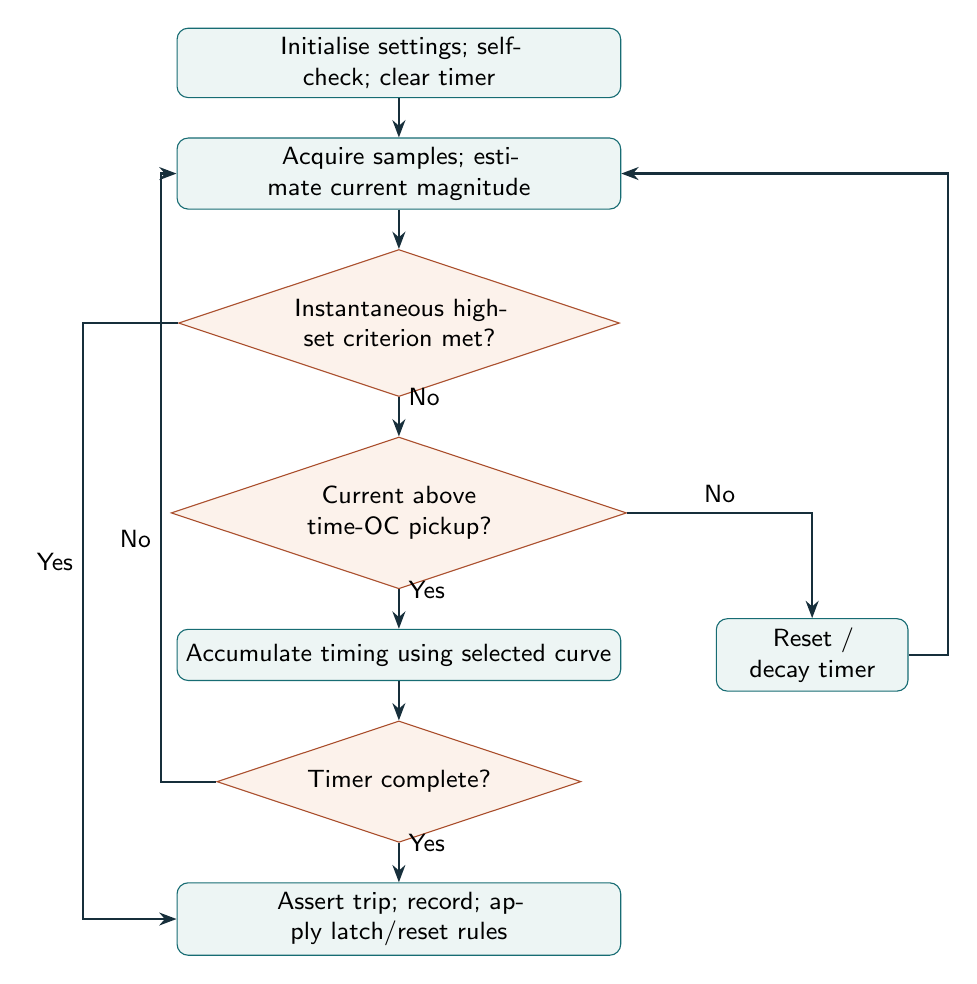
\begin{tikzpicture}[node distance=5mm,font=\small\sffamily,
 proc/.style={draw=teal,fill=pale,rounded corners,text width=5.4cm,align=center,minimum height=.65cm},
 dec/.style={diamond,aspect=3,draw=rust,fill=warm,text width=3.5cm,align=center,inner sep=1pt}]
\node[proc] (st){Initialise settings; self-check; clear timer};
\node[proc,below=of st] (sa){Acquire samples; estimate current magnitude};
\node[dec,below=of sa] (hi){Instantaneous high-set criterion met?};
\node[dec,below=of hi] (pi){Current above time-OC pickup?};
\node[proc,below=of pi] (ti){Accumulate timing using selected curve};
\node[dec,below=of ti] (do){Timer complete?};
\node[proc,below=of do] (tr){Assert trip; record; apply latch/reset rules};
\foreach \a/\b in {st/sa,sa/hi,hi/pi,pi/ti,ti/do,do/tr}{\draw[arr] (\a)--(\b);}
\node[proc,text width=2.2cm,right=12mm of ti] (rs){Reset / decay timer};
\draw[arr] (pi.east)-|(rs.north)node[pos=.25,above]{No};
\draw[arr] (rs.east)--++(.5,0)|-(sa.east);
\draw[arr] (hi.west)--++(-1.2,0)|-(tr.west)node[pos=.2,left]{Yes};
\draw[arr] (do.west)--++(-.7,0)|-(sa.west)node[pos=.2,left]{No};
\node[right] at (hi.south){No};\node[right] at (pi.south){Yes};\node[right] at (do.south){Yes};
\end{tikzpicture}\end{center}
\diagramcaption{Educational 50/51 decision flow. Repeated acquisition is continuous; reset, supervision and latching follow the specified relay algorithm.}
For a constant overcurrent, a definite-time implementation counts elapsed samples. For changing current with an inverse curve, one useful educational accumulator is
\[
 q\leftarrow q+\frac{\Delta t}{t(M)},\qquad\text{trip when }q\ge1.
\]
This models progress toward operation rather than restarting a full timer every sample. Below pickup, the chosen reset rule clears or decays $q$. The source flowchart uses an initial threshold/delay, repeated checking, time setting and execution of trip; the more explicit chart above makes the continuing pickup and reset decisions visible.

\subsubsection{Original microprocessor flowchart}\slides{Protection, p. 66}
\begin{center}\includegraphics[width=.94\textwidth,height=68mm,keepaspectratio]{Study_Assets/Module3/pr_066.pdf}\end{center}
\diagramcaption{Follow acquisition, pickup decision, delay, repeated current check, trip and reset. The main text adds explicit dropout handling and a clearer loop.}

\subsection{Fundamentals of a numerical relay}
A numerical relay implements measurements and protection algorithms on digitally represented samples, often with a microprocessor/DSP. ``Microprocessor'' and ``numerical'' overlap in practice: an early processor-based relay may make simple magnitude/time decisions; numerical systems commonly provide sampled-waveform estimation and many functions. They are not completely separate physical principles.

An anti-alias filter limits high-frequency components before sampling. The Nyquist condition alone is not a complete relay design; filter response, sampling rate, estimator window and fault transients matter. Fundamental-frequency phasors may be estimated with a DFT or other algorithms. ADC range/resolution, CT saturation, frequency deviation, DC offset and harmonics influence measurement; filtering is not a guarantee to remove every error.

Typical functions include programmable OC/directional/distance/differential elements, event and waveform recording, metering, setting groups, self-diagnostics, breaker monitoring, communications and logic. Advantages include repeatable characteristics, multifunction capability and easier records/settings management. Limitations include dependence on auxiliary power and correct firmware/settings, possible common hardware/software failures, measurement transients and the need for secure access and testing. Self-diagnostics detect some faults, not every failure.

The slides' 16--64 samples/cycle, 0.01-step settings, specific chassis sizes and proprietary logic examples describe particular implementations, not all numerical relays. IEC 61850 provides substation communication/data-model capabilities; using it does not automatically guarantee speed, redundancy or cybersecurity. Adaptive/AI-based functions are contextual material, not a replacement for understanding the deterministic protection conditions in this module.

\subsubsection{Sample-and-hold numerical hardware}\slides{Protection, p. 72}
\begin{center}\includegraphics[width=.94\textwidth,height=68mm,keepaspectratio]{Study_Assets/Module3/pr_072.pdf}\end{center}
\diagramcaption{CT/VT signals are conditioned, sampled, multiplexed, converted and processed. Anti-alias filtering is explained in the main text.}

\subsubsection{Numerical relay signal and power paths}\slides{Protection, p. 73}
\begin{center}\includegraphics[width=.94\textwidth,height=68mm,keepaspectratio]{Study_Assets/Module3/pr_073.pdf}\end{center}
\diagramcaption{Surge filtering and anti-alias filtering protect the analogue input; the processor runs protection logic and sends digital outputs and communications.}
\begin{center}\small
\begin{tabularx}{\textwidth}{L{.18\textwidth}L{.23\textwidth}L{.23\textwidth}Y}
\toprule Feature & Induction electromechanical & Static analogue & Numerical\\\midrule
Decision & Flux, torque, moving disc/cup & Electronic comparator/timer & Sampled values + software\\
Timing settings & Tap, dial; construction curve & Electronic references/RC circuit & Pickup, curve, TMS and reset logic\\
Records / functions & Usually limited & Usually limited by circuitry & Commonly multiple functions and stored records\\
What can still move? & Disc/cup and contacts & Output relay / breaker & Output contacts / breaker\\
Key checks & Mechanical condition, pickup/timing & Supply, drift, surge immunity & Supply, settings, firmware, input/logic performance\\\bottomrule
\end{tabularx}\end{center}

\chapterstart{Circuit breakers and the arc-extinction problem}{breakers}
\slides{Syllabus supplement: Module 3 circuit-breaker items on syllabus PDF p. 2. The supplied protection deck provides relay/trip context but no dedicated breaker section.}
\subsection{What the breaker must accomplish}
A circuit breaker makes, carries and interrupts current within its assigned ratings, including specified fault duties. Its closed contacts offer a low-resistance conducting path. A trip command releases an operating mechanism so contacts separate; successful interruption requires the conducting arc to die and the contact gap to remain insulating under the voltage that returns across it.

The trip coil generally releases stored operating energy; the coil need not itself supply all contact-separation energy. Breaker \emph{opening time} runs to contact separation; \emph{arcing time} runs from arc initiation to final extinction; their sum after the applicable initiation defines interruption time according to the stated convention. Fault clearing also includes preceding relay delays. These intervals should not be counted twice.

An isolator/disconnector establishes isolation under its specified switching duties; it is not a substitute for a fault-interrupting circuit breaker. A fuse interrupts by melting its element and extinguishing its arc, and normally must be replaced after operation. The breaker can be operated again after the fault and its condition/duty permit it.
\subsection{Why opening contacts initially produces an arc}
At separation the last contact area becomes small, current density and local temperature increase, and a conducting plasma path can form. Gas ionisation and/or vaporised contact material sustain the arc depending on the medium. Current continues after the metal contacts have separated. Inductance resists abrupt current change; the circuit can produce a high voltage if interruption attempts a rapid $di/dt$:
\[
 v_L=L\frac{di}{dt},\qquad W_L=\tfrac12Li^2.
\]
The arc converts electrical energy to heat. Its voltage, current, contact geometry and cooling determine its behaviour; it is not simply a fixed resistor. A wider gap alone does not prove that the arc will extinguish or remain extinguished.
\subsection{The two elementary arc-extinction approaches}
\textbf{High-resistance method:} increase the arc's effective resistance/voltage enough to force its current down. Cooling, lengthening, narrowing/constriction and splitting into multiple series arcs are familiar methods. Arc chutes and magnetic movement can assist suitable devices. The method dissipates energy and can produce switching overvoltage; application depends on the switch design and circuit duty, and is associated with many lower-voltage/current-limiting and DC interruption arrangements.

\textbf{Low-resistance / current-zero method:} in an AC breaker, allow the arc to conduct until a natural current zero, then rapidly restore insulation so current does not restart. The arc need not be forced to a very high resistance throughout the preceding half-cycle. Cooling, removal of hot ionised material, recombination, electron attachment in suitable gases, or rapid loss/condensation of conducting vapour help the post-zero gap recover.

\Needspace{5\baselineskip}
The term ``low resistance'' describes the conducting arc before extinction; it does not mean the open breaker should have a low resistance. Both methods manage heat, charge carriers and recovery voltage. AC natural-current-zero interruption is central to the SF$_6$ and VCB explanations below. DC has no periodic natural current zero and needs a suitable dedicated interruption/current-zero-creation mechanism; an AC rating cannot simply be reused for DC.

\subsection{Current zero, recovery voltage and the race for insulation}
Near AC current zero, energy input to the arc is reduced and the conductive channel can collapse. The network then applies a voltage across the separating contacts. The immediate transient is \textbf{transient recovery voltage (TRV)}; after transients subside, the power-frequency voltage across the open gap is the recovery voltage. Traditional texts often use ``restriking voltage'' for the initial transient. Actual reignition/restrike means conduction restarts because interruption failed at that stage.

Success requires both:
\begin{itemize}
\item \textbf{Thermal recovery:} residual post-arc current and remaining heating must not rebuild the hot conducting path immediately after zero.
\item \textbf{Dielectric recovery:} the recovering gap's withstand capability must remain above the applied recovery-voltage stress as time progresses.
\end{itemize}
A common introductory description compares rate of rise of recovery voltage with rate of dielectric recovery; the full voltage-versus-time curves and thermal behaviour matter, not just one slope. TRV depends on circuit inductance, capacitance, source/fault location and switching conditions.
\begin{center}
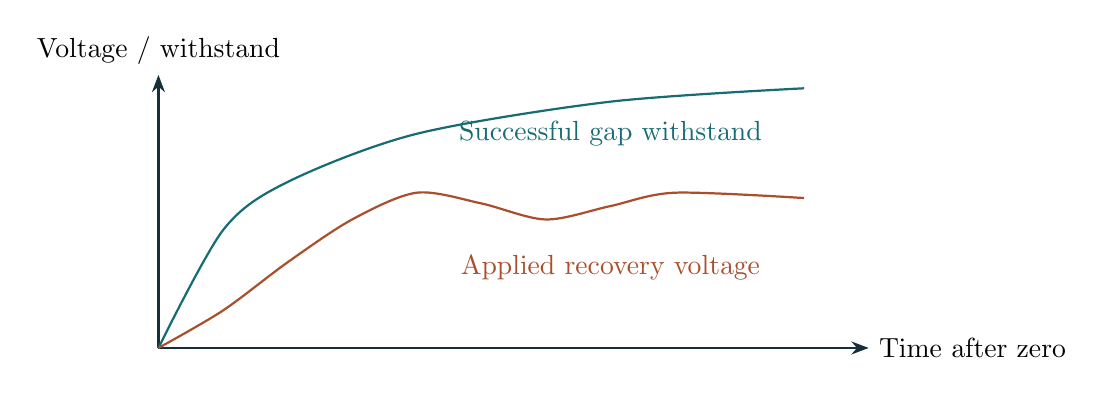
\begin{tikzpicture}[x=.82cm,y=.68cm]
\draw[arr] (0,0)--(11,0)node[right]{Time after zero};\draw[arr] (0,0)--(0,5.1)node[above]{Voltage / withstand};
\draw[teal,thick] plot[smooth] coordinates{(0,0)(1,2.2)(2,3.1)(4,4)(7,4.6)(10,4.85)};
\draw[rust,thick] plot[smooth] coordinates{(0,0)(1,.7)(2,1.6)(3,2.4)(4,2.9)(5,2.7)(6,2.4)(7,2.65)(8,2.9)(10,2.8)};
\node[teal] at (7,4){Successful gap withstand};\node[rust] at (7,1.5){Applied recovery voltage};
\end{tikzpicture}\end{center}
\diagramcaption{Conceptual successful interruption: withstand exceeds applied stress. Not a measured or standardised TRV test waveform; near-zero thermal recovery must also succeed.}

\subsection{An optional elementary LC recovery-voltage derivation}
This derivation helps explain the source of a transient; it is not an additional numerical requirement in the supplied syllabus. Consider a simplified lossless source-side circuit after current zero: approximately constant source voltage $E_m$ over the short transient, inductance $L$ and effective capacitance $C$ across the open break. With $v_C(0)=0$, $i(0)=0$,
\[
 L\frac{di}{dt}+v_C=E_m,\quad i=C\frac{dv_C}{dt}
 \quad\Rightarrow\quad LC\frac{d^2v_C}{dt^2}+v_C=E_m.
\]
The solution is
\[
 v_C(t)=E_m[1-\cos(\omega_0t)],\qquad \omega_0=1/\sqrt{LC}.
\]
The first ideal peak is $2E_m$ at $t=\pi/\omega_0$. Average rise to this peak is $2E_m\omega_0/\pi$; maximum instantaneous slope is $E_m\omega_0$. The initial derivative in this special model is zero, so the average rise is not the derivative at $t=0$. Real damping and distributed network dynamics change the waveform and peaks; do not treat $2E_m$ as every breaker TRV.

\subsection{Current chopping and reclosing context}
\textbf{Current chopping} interrupts a small inductive current before its natural zero. The stored inductive energy can charge capacitance and cause overvoltage. An ideal energy estimate is
\[
 \tfrac12LI_{ch}^2=\tfrac12C(\Delta V)^2
 \quad\Rightarrow\quad \Delta V\approx I_{ch}\sqrt{L/C},
\]
under the deliberately simplified zero-initial-capacitor-voltage, lossless model. Contact material, design and suitable surge protection reduce troublesome effects. Chopping, restrike and normal current-zero interruption are different concepts.

Automatic reclosing may restore supply after a transient line fault; permanent faults require lockout according to the scheme. A breaker must withstand its specified operating duty, fault making, interruption and repeated operations. Relay reset/trip-latch logic and breaker readiness therefore belong to the overall protection chain.

\subsection{Classification and key ratings}
By arc-extinction medium, elementary classifications include oil (bulk/minimum oil), air/air blast, SF$_6$/other gas, and vacuum. By construction, live-tank and dead-tank arrangements distinguish whether the interrupter enclosure is at line potential or earth potential. These are different classification axes. The syllabus asks detailed study of SF$_6$ and vacuum.

Key ratings include rated voltage and insulation withstand, continuous current, short-circuit breaking current, peak making current, short-time withstand current and specified operating duty/TRV capability. Breaking current is commonly stated as an RMS symmetrical component with specified conditions; peak making duty accounts for asymmetry. The old three-phase breaking-capacity expression
\[
 S_{break}(\mathrm{MVA})=\sqrt3V_{rated}(\mathrm{kV})I_{break}(\mathrm{kA})
\]
expresses a duty convention, not actual useful power delivered into a bolted fault. Practical selection requires all applicable ratings rather than MVA alone.

\chapterstart{SF6 and vacuum circuit breakers}{sfvac}
\slides{Syllabus supplement; primary technical references are linked in Section~\ref{coverage}.}
\subsection{SF6: gas insulation and current-zero interruption}
Sulphur hexafluoride (SF$_6$) provides strong insulation and useful arc-interruption properties. It is electronegative: capture of free electrons helps reduce conducting charge carriers in the recovering gas. Cooling and replacement/removal of hot arc gas are also essential; electron attachment alone is not the complete interruption mechanism.

An elementary \textbf{puffer} interrupter contains fixed/moving main contacts, arcing contacts, an insulating nozzle and a gas compression chamber/piston associated with the operating mechanism. The opening movement compresses gas and directs it through the arcing region. Main contacts carry normal current and separate before the arcing contacts; the latter carry the arc. Self-blast/thermal-assisted designs use arc energy to assist gas pressure and reduce mechanism energy for suitable duties.
\begin{center}
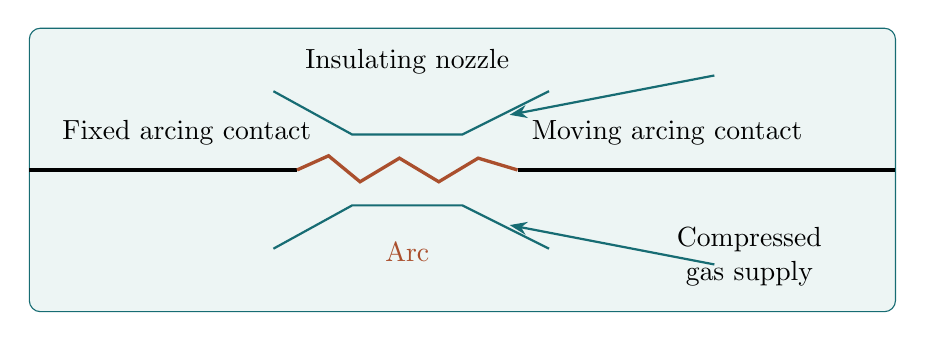
\begin{tikzpicture}
\draw[teal,rounded corners,fill=pale] (0,-1.8)rectangle(11,1.8);
\draw[very thick] (0,0)--(3.4,0);\draw[very thick] (6.2,0)--(11,0);
\draw[rust,very thick] (3.4,0)--(3.8,.18)--(4.2,-.15)--(4.7,.15)--(5.2,-.15)--(5.7,.15)--(6.2,0);
\draw[teal,thick] (3.1,1)--(4.1,.45)--(5.5,.45)--(6.6,1);
\draw[teal,thick] (3.1,-1)--(4.1,-.45)--(5.5,-.45)--(6.6,-1);
\node[above] at (2,.2){Fixed arcing contact};\node[above] at (8.1,.2){Moving arcing contact};
\node[above] at (4.8,1.1){Insulating nozzle};\node[below,rust] at (4.8,-.8){Arc};
\draw[arr,teal] (8.7,1.2)--(6.1,.7);\draw[arr,teal] (8.7,-1.2)--(6.1,-.7);
\node[right,align=center] at (8.1,-1.1){Compressed\\gas supply};
\end{tikzpicture}\end{center}
\diagramcaption{Functional puffer gas-flow sketch, not a detailed engineering cross-section. The separate main-contact path and compression piston are omitted for clarity.}
\textbf{Opening sequence:} trip releases the mechanism; main contacts separate and current transfers to the arcing path; arcing contacts part and an arc forms; gas compression/nozzle flow cools the channel and carries hot products away; at current zero the gap recovers; continuing contact travel and cool insulating gas allow it to withstand TRV. Reignition is possible if gas flow or recovery is inadequate. This sequence is cross-checked against Schneider Electric's puffer explanation and ABB's breaker description.

Advantages include effective interruption/insulation and compact arrangements for suitable duties, without oil as the interrupting medium. Limitations include sealed-gas-system requirements, pressure/density monitoring, leakage management and handling of arc decomposition products. SF$_6$ is a strong greenhouse gas; containment, recovery and reduced-emission alternatives matter. No specific regulatory rule or future phase-out date is asserted here.

\subsection{VCB: a metal-vapour arc in a sealed vacuum interrupter}
A vacuum circuit breaker uses a hermetically sealed interrupter with fixed and moving contacts, insulating envelope (often ceramic), metal end seals, a flexible metal bellows for moving-contact travel and an internal vapour shield. The vacuum is the interrupting environment; the whole switchgear assembly still requires external insulation.
\begin{center}
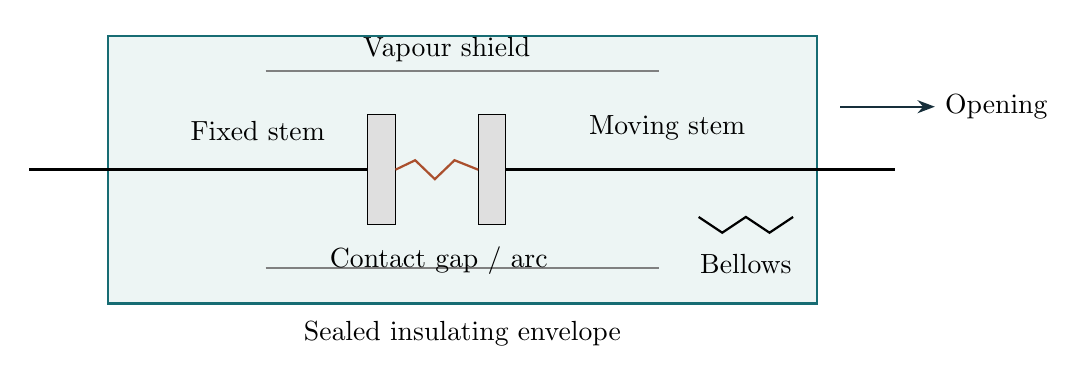
\begin{tikzpicture}
\draw[teal,thick,fill=pale] (1,-1.7)rectangle(10,1.7);
\draw[gray,thick] (3,-1.25)--(8,-1.25);\draw[gray,thick] (3,1.25)--(8,1.25);
\draw[very thick] (0,0)--(4.3,0);\draw[fill=gray!25] (4.3,-.7)rectangle(4.65,.7);
\draw[fill=gray!25] (5.7,-.7)rectangle(6.05,.7);\draw[very thick] (6.05,0)--(11,0);
\draw[rust,thick] (4.65,0)--(4.9,.12)--(5.15,-.12)--(5.4,.12)--(5.7,0);
\draw[thick] (8.5,-.6)--(8.8,-.8)--(9.1,-.6)--(9.4,-.8)--(9.7,-.6);
\node[above] at (2.9,.25){Fixed stem};\node[above] at (8.1,.25){Moving stem};
\node[above] at (5.3,1.25){Vapour shield};\node[below] at (5.2,-.85){Contact gap / arc};
\node[below] at (9.1,-.95){Bellows};\node[below] at (5.5,-1.8){Sealed insulating envelope};
\draw[arr] (10.3,.8)--(11.5,.8)node[right]{Opening};
\end{tikzpicture}\end{center}
\diagramcaption{Labelled conceptual vacuum bottle. Bellows representation is schematic; it preserves a vacuum seal while allowing axial movement.}
Vacuum does \emph{not} mean no arc can form. Contact separation produces metal vapour from the electrodes, which supplies the conducting plasma. Suitable contact geometry can use magnetic fields to distribute arc energy and avoid local overheating. Near current zero, the vapour arc can no longer be sustained; vapour rapidly condenses on internal metal surfaces and the contact gap recovers dielectric strength. This mechanism is cross-checked against Siemens' vacuum-interrupter technical descriptions.

Advantages include a short required contact gap, rapid dielectric recovery, low arc energy and a sealed interrupting unit without an SF$_6$ gas-interruption system. Vacuum interrupters are widely used in medium-voltage applications and suitable specialised duties; there is no universal maximum voltage to memorise independently of device design.

Limitations/considerations include vacuum integrity, contact erosion and switching duty, current-chopping/restrike overvoltages for some inductive loads, and suitable protection/insulation coordination. A sealed interrupter may require replacement rather than internal field repair. The mechanism, connections and external insulation still need maintenance/checks even when the vacuum bottle is described as maintenance-free.

\subsection{Comparison that can be written in an exam}
\begin{center}\small\renewcommand{\arraystretch}{1.08}
\begin{tabularx}{\textwidth}{L{.24\textwidth}L{.34\textwidth}Y}
\toprule Aspect & SF$_6$ breaker & Vacuum breaker\\\midrule
Interrupting environment & Controlled insulating gas & Sealed evacuated chamber\\
Arc medium & Hot ionised gas with electrode products & Primarily contact-metal vapour\\
Extinction emphasis & Gas flow cools the arc; insulation recovers at current zero & Vapour plasma collapses/condenses; gap recovers at current zero\\
Core construction & Arcing/main contacts, nozzle, compression chamber & Contacts, sealed envelope, bellows, vapour shield\\
System considerations & Gas density, leakage and decomposition products; greenhouse impact & Vacuum seal/contact condition; inductive-load switching overvoltage\\
External insulation & External insulation still required & External insulation still required\\\bottomrule
\end{tabularx}\end{center}
\checkq{What must happen after the arc reaches current zero?}{The conducting channel must lose conductivity, and the gap must recover enough dielectric strength to withstand the returning voltage. Current zero alone does not guarantee interruption.}

\chapterstart{Additional integrated practice}{integrated}
\subsection{From nameplate reactance to bus fault current}
A 25 MVA, 11 kV generator with $X_d''=0.20$ p.u. feeds an 11/66 kV transformer rated 25 MVA with $X_T=0.10$ p.u.; a line has $X_L=20\ \Omega$/phase on the 66 kV side. Find solid three-phase fault current at the far end, neglecting load/resistance and assuming $E=1$. Select system base 50 MVA, 11/66 kV.
\[
 X_G=0.20(50/25)=0.40,\quad X_T=0.10(50/25)=0.20,\quad
 Z_{B,66}=66^2/50=87.12\ \Omega,
\]
\[
 X_L=20/87.12=0.2295684,\quad X_{1,eq}=0.8295684,\quad
 |I_f|=1/0.8295684=1.205446\ \mathrm{p.u.}
\]
\[
 I_{B,66}=50/(\sqrt3\,66)=0.4373866\ \mathrm{kA},\quad
 \ans{|I_f|=0.527246\ \mathrm{kA}}.
\]
Short-circuit level is $50/0.8295684=60.2723$ MVA. The answer is far-end current at 66 kV; multiplying by the 11 kV base current instead would give the referred generator-side current, a different quantity. No additional ideal-ratio impedance appears in the p.u. series sum.
\subsection{Finite ground-fault resistance changes both magnitude and angle}
At a bus, $E=1$, $Z_1=\jj0.2$, $Z_2=\jj0.2$, $Z_0=\jj0.1$ p.u. An $a$-ground fault has \emph{resistance} $Z_f=0.05$ p.u. Then
\[
 I_1=\frac1{0.15+\jj0.5}=0.550459-\jj1.834862,
\]
\[
 \ans{I_a=1.651376-\jj5.504587\ \mathrm{p.u.}},\quad
 |I_a|=5.746958\ \mathrm{p.u.},\quad \angle I_a\approx-73.3008^\circ.
\]
$V_a=Z_fI_a=0.0825688-\jj0.2752294$ p.u. All three sequence currents are equal; the unfaulted fault-branch currents remain zero. Resistance cannot be inserted as another imaginary reactance.
\subsection{A relay-trip decision with a specified reset rule}
For a definite-time OC element, pickup is 400 A primary and delay is 0.30 s. Current is 600 A for 0.18 s, then 350 A for 0.05 s, then 600 A for 0.20 s. With \emph{instantaneous timer reset} below pickup, neither above-pickup interval reaches 0.30 s; there is no delayed trip. If the problem instead specifies a slow-decay reset, the answer can change. This is why a numerical relay's reset setting belongs in the coordination model.

\chapterstart{Revision sheets and error-proof workflows}{revision}
\subsection{Base quantities and sequence transformation}
\begin{Idea}{Keep these conventions on every calculation page}
Three-phase base uses \emph{total} $S_B$ and \emph{line-to-line} $V_B$:
\[
 I_B=\frac{S_B}{\sqrt3V_B},\quad Z_B=\frac{V_B^2}{S_B},\quad
 Z_{\rm pu,new}=Z_{\rm pu,old}\frac{S_{B,new}}{S_{B,old}}
 \left(\frac{V_{B,old}}{V_{B,new}}\right)^2.
\]
Keep $S_B$ common throughout the network and choose voltage bases across each transformer in its rated line-voltage ratio. Each zone has its own $I_B$ and $Z_B$.
\[
 a=-\frac12+\jj\frac{\sqrt3}{2},\quad a^2=-\frac12-\jj\frac{\sqrt3}{2},\quad
 a^3=1,\quad 1+a+a^2=0.
\]
\[
 \begin{bmatrix}I_0\\I_1\\I_2\end{bmatrix}
 =\frac13\begin{bmatrix}1&1&1\\1&a&a^2\\1&a^2&a\end{bmatrix}
 \begin{bmatrix}I_a\\I_b\\I_c\end{bmatrix},\qquad
 \begin{bmatrix}I_a\\I_b\\I_c\end{bmatrix}
 =\begin{bmatrix}1&1&1\\1&a^2&a\\1&a&a^2\end{bmatrix}
 \begin{bmatrix}I_0\\I_1\\I_2\end{bmatrix}.
\]
Replace $I$ by $V$ for voltages. The factor $1/3$ belongs to the phase-to-sequence transformation. $I_a+I_b+I_c=3I_0$ is the residual/earth-return current under the chosen reference direction.
\end{Idea}
\subsection{Fault equations on one page}
Use common-base Thevenin impedances at the fault bus. In every row,
\[
 V_1=E-Z_1I_1,\qquad V_2=-Z_2I_2,\qquad V_0=-Z_0I_0.
\]
\begin{center}\small
\begin{tabularx}{\textwidth}{L{.12\textwidth}L{.43\textwidth}Y}
\toprule Fault & Sequence-current equation & Phase condition / connection\\\midrule
3-phase solid & $I_1=E/Z_1$, $I_0=I_2=0$ & Positive network only; $I_a=I_1$, $I_b=a^2I_1$, $I_c=aI_1$.\\
$a$-ground & $I_0=I_1=I_2=E/(Z_1+Z_2+Z_0+3Z_f)$ & Three sequence networks in series; $I_a=3I_1$; $I_b=I_c=0$; $V_a=Z_fI_a$.\\
$b$-$c$ & $I_1=E/(Z_1+Z_2+Z_f)$, $I_2=-I_1$, $I_0=0$ & $I_a=0$, $I_b=-\jj\sqrt3 I_1$, $I_c=-I_b$; $Z_f$ is impedance between the faulted phases.\\
$b$-$c$-ground & $I_1=\displaystyle\frac{E}{Z_1+\frac{Z_2(Z_0+3Z_f)}{Z_2+Z_0+3Z_f}}$ & Positive network feeding negative and modified zero networks in parallel; $Z_f$ is the common path to ground.\\
 & $I_2=-I_1\displaystyle\frac{Z_0+3Z_f}{Z_2+Z_0+3Z_f}$ & $I_a=0$; $V_b=V_c=Z_f(I_b+I_c)$.\\
 & $I_0=-I_1\displaystyle\frac{Z_2}{Z_2+Z_0+3Z_f}$ & Reconstruct $I_b,I_c$ using the full inverse transformation.\\\bottomrule
\end{tabularx}\end{center}
For the solid LL case, $V_1=V_2$ and $V_0=0$. For the solid LLG case, $V_0=V_1=V_2$; these equal values are \emph{sequence terminal voltages}, not three phase voltages. For LG with a disconnected zero-sequence network, the ideal steady-state sequence model gives no metallic earth-fault path; capacitances may still permit current in a more complete model.

\subsection{A six-step fault-analysis routine}
\begin{enumerate}
\item Draw the one-line network, mark the faulted bus and identify connections/grounding. State fault type, phase labels, fault impedance and whether load is neglected.
\item Select a common power base and compatible voltage bases. Convert every impedance before combining it. Include $3Z_n$ in the zero-sequence neutral path.
\item Draw positive, negative and zero networks, retaining only physically available zero-sequence paths. Reduce each to the driving-point Thevenin equivalent at the fault bus.
\item Apply phase boundary conditions to connect the sequence networks. Calculate $I_0,I_1,I_2$ as \emph{complex} quantities, including their signs.
\item Reconstruct phase currents and, if requested, sequence and phase voltages. Convert to amperes with the current base \emph{at the fault location}.
\item Check the unfaulted fault-branch currents, equal/opposite LL currents, earth-current sum, and voltage conditions. Round only the final result.
\end{enumerate}
\begin{Caution}{Checks that catch most mistakes}
$1/(\jj X)=-\jj/X$, but $-V/(\jj X)=+\jj V/X$. A sign error in the second expression corrupts an LLG reconstruction. In a $b$-$c$-ground fault, $I_a$ must be zero in the fault branch; $3I_0$ is the total earth current, not automatically one faulted-phase current. A computed $I_a\ne0$ is a failed boundary condition, even if another magnitude looks plausible.
\end{Caution}
\subsection{Protection decisions to recognise immediately}
\begin{center}\small
\begin{tabularx}{\textwidth}{L{.18\textwidth}L{.40\textwidth}Y}
\toprule Principle & Decision quantity & Essential check\\\midrule
Overcurrent & $M=I/I_{pickup}$; trip after selected time if $M>1$ & Load allowance, minimum fault sensitivity, downstream coordination.\\
Directional OC & Directional voltage/current comparison enables OC & Reference polarity and polarising signal during the relevant fault.\\
Distance & Compensated fault-loop $Z_{app}=V_{loop}/I_{loop}$ & Correct loop, CT/VT conversion, reach, infeed and fault resistance.\\
Differential & $I_{op}=|I_1-I_2|$ after ratio/polarity compensation & External-fault stability; CT saturation, bias, transformer inrush.\\\bottomrule
\end{tabularx}\end{center}
For the standard inverse example used here,
\[
 t=TMS\frac{0.14}{M^{0.02}-1}\quad(M>1).
\]
Curve family, time multiplier, pickup, reset rule and instantaneous setting all matter. Primary and backup protection are \emph{roles}; induction, static and numerical are \emph{technologies}; OC/distance/differential are \emph{principles}. Do not mix these classifications.

For a circuit breaker, the relay orders a trip, the mechanism separates contacts, an arc carries current temporarily, and the interrupting medium must remove conductivity and withstand the returning voltage. In an AC breaker, the decisive interval lies around current zero. SF$_6$ uses controlled gas action; a VCB extinguishes a contact-metal-vapour arc inside an evacuated interrupter.
\subsection{Common confusions: make the distinction explicit}
\begin{center}\small
\begin{tabularx}{\textwidth}{L{.42\textwidth}Y}
\toprule Tempting shortcut & Correct interpretation\\\midrule
Use line voltage with per-phase VA in $V^2/S$ & Use line voltage with total three-phase VA, or phase voltage with per-phase VA.\\
All equipment reactances can be added as given & Nameplate p.u. values must first use a common base.\\
A delta blocks every zero-sequence effect & It blocks external zero-sequence line current on that side; internal circulation can support a grounded-wye-side path.\\
Negative sequence has a separate generator EMF & The balanced pre-fault source exists in the positive network; negative and zero networks are passive in this model.\\
Fault always means the largest possible current & High-impedance faults and weak infeed can produce limited current; three-phase need not be the largest fault.\\
An instantaneous element takes zero seconds & It has no intentional delay; measuring, output and breaker times remain.\\
An induction relay works from one alternating flux alone & Net average induction torque needs two spatially and temporally displaced fluxes.\\
A microprocessor OC relay is a complete modern numerical relay & It is one implementation/function; modern multifunction numerical relays extend measurement, logic and supervision.\\
An isolator can interrupt the short circuit & A conventional isolator provides isolation after interruption; fault interruption requires a suitably rated breaker.\\
No air in a VCB means no arc & Contact-metal vapour forms the arc during interruption.\\\bottomrule
\end{tabularx}\end{center}

\chapterstart{Exam practice with answers}{practice}
\subsection{How to use the supplied examination pattern}
The syllabus specifies a 60-mark, 2 hour 30 minute end-semester examination. Part A has eight compulsory 3-mark questions, two from each module, totalling 24 marks. Part B offers two 9-mark full questions from each module; answer one from each pair, totalling 36 marks. A full question has at most three subparts. The prompts below follow those sizes for practice; they are not claimed predictions or past-paper questions.

For a numerical answer, give the base, equivalent network, formula, complex substitution and units. For a descriptive answer, start with the operating quantity, draw and label the diagram, explain the sequence of operation, and mention the important limitation. A labelled diagram plus a connected explanation earns more confidence than an isolated list of component names.
\subsection{Three-mark self-test: attempt before reading the answer}
\checkq{1. Derive three-phase impedance base using line quantities.}{Using $V_{B,ph}=V_{B,LL}/\sqrt3$ and $S_{B,ph}=S_B/3$, $Z_B=V_{B,ph}^2/S_{B,ph}=V_{B,LL}^2/S_B$. The current base remains $S_B/(\sqrt3V_{B,LL})$.}
\checkq{2. Give two benefits and one condition of the per-unit method.}{It simplifies transformer referral and puts differently rated equipment on comparable normalised scales. The condition is a common system power base with transformer-compatible voltage bases; convert old apparatus bases first.}
\checkq{3. Define positive, negative and zero sequence.}{Positive sequence is an equal-magnitude balanced set in the chosen $a$-$b$-$c$ order; negative sequence has the reverse order. Zero-sequence phasors are equal in magnitude and phase, so their sum is three times one component.}
\checkq{4. Why does neutral impedance enter as $3Z_n$?}{Each zero-sequence phase current equals $I_0$; the neutral carries $3I_0$. Its voltage drop $3I_0Z_n$ contributes an equivalent $3Z_n$ in the per-phase zero network.}
\checkq{5. State the boundary conditions and sequence connection for an LG fault.}{$I_b=I_c=0$ and $V_a=Z_fI_a$. Thus $I_0=I_1=I_2$; the three sequence networks are in series with $3Z_f$. For a solid fault, $V_a=0$.}
\checkq{6. Why is zero sequence absent from a pure LL fault?}{No current flows in the unfaulted phase and the two faulted-phase currents are equal and opposite. Their sum is zero, so $I_0=(I_a+I_b+I_c)/3=0$.}
\checkq{7. Distinguish primary and backup protection.}{Primary protection normally clears faults in the intended protected zone. Backup acts if the primary relay, its trip chain or breaker fails; it may use independent local equipment or delayed remote protection, often with less selectivity.}
\checkq{8. What makes a protection scheme selective and sensitive?}{Selectivity confines disconnection to the equipment required to isolate the fault. Sensitivity ensures operation for the lowest relevant fault signal while remaining secure under load and permissible transients. Settings must balance both objectives.}
\checkq{9. Explain induction-relay torque in one equation.}{$T\propto\Phi_1\Phi_2\sin\delta$: AC fluxes displaced in space and time induce eddy currents whose interactions produce net torque. For a current-operated arrangement with fluxes proportional to current, operating torque is approximately proportional to $I^2$.}
\checkq{10. Give the functional blocks of a static instantaneous OC relay.}{CT/input conversion $\rightarrow$ rectification or conditioning $\rightarrow$ pickup comparator $\rightarrow$ output driver/trip contact. A reference establishes pickup; there is no intentional timing stage, although finite processing/output time remains.}
\checkq{11. What blocks protect a numerical relay from misleading samples?}{Input isolation/conditioning, an analogue anti-alias filter and appropriate sampling precede digital estimation. The processor checks signals and applies settings/logic. Filtering cannot by itself repair saturated CT information or an incorrect CT ratio/polarity.}
\checkq{12. State the distance and differential principles.}{Distance estimates impedance from an appropriate voltage/current fault loop and compares it with a reach characteristic. Differential compares compensated currents at a zone's boundaries; substantial imbalance indicates an internal fault, with restraint for measurement error and through-current.}
\checkq{13. Why is current zero necessary but insufficient for AC interruption?}{The arc receives no instantaneous current input at zero, permitting conductivity to collapse. The contact gap must then recover quickly enough to withstand TRV; otherwise conduction can resume.}
\checkq{14. Compare the arc media of SF$_6$ and VCB.}{SF$_6$ interruption uses gas-flow cooling and rapid insulation recovery, aided by the gas's electron attachment. Vacuum interruption involves contact-metal-vapour plasma; around current zero the vapour/plasma collapses and condenses, allowing rapid gap recovery.}
\subsection{Numerical drill: questions}
\begin{enumerate}[label=\textbf{N\arabic*.}]
\item On a 100 MVA, 11 kV base, find $I_B$ and $Z_B$. Express $\jj0.2$ p.u. in ohms.
\item Convert $0.15$ p.u. on 25 MVA, 11 kV to 50 MVA, 13.2 kV at the \emph{same physical terminals}.
\item Find the sequence components of $I_a=30$, $I_b=30\angle120^\circ$, $I_c=30\angle-120^\circ$ A.
\item $E=1$, $Z_1=\jj0.2$, $Z_2=\jj0.3$, $Z_0=\jj0.1$ p.u. Find solid $a$-ground fault current and sequence currents. Is it larger than the solid three-phase current?
\item For the same impedances, find solid $b$-$c$ fault phase currents and sequence voltages.
\item For the same impedances, find solid $b$-$c$-ground sequence currents, both faulted-phase currents, and total earth current. Check $I_a$.
\item A CT is 600/5 A. The OC pickup setting is 125\% of the 5 A relay rating. At 3000 A primary, find secondary current, primary pickup and pickup multiple. For the standard inverse curve with TMS $=0.1$, find operating time.
\item A protected line is $5+\jj20\ \Omega$ primary. Zone 1 is set to 80\%. CT ratio is 500/5 and VT ratio is 110000/110. Find the secondary relay reach.
\item In a compensated differential convention, $I_1=8$, $I_2=7.2$ A. Use $I_{op}>0.2+0.25I_{bias}$ with $I_{bias}=(|I_1|+|I_2|)/2$. Does the element operate? Repeat for $I_1=8$, $I_2=2$ A.
\item A downstream relay trips in 0.15 s, its breaker clears in 0.06 s, and grading margin is 0.10 s. Find the minimum upstream relay operating time under the specified coordination rule.
\end{enumerate}
\subsection{Numerical drill: answers and checks}
\begin{enumerate}[label=\textbf{N\arabic*.}]
\item $I_B=100/(\sqrt3\,11)=5.248639$ kA; $Z_B=11^2/100=1.21\ \Omega$; actual reactance is $\jj0.242\ \Omega$/phase.
\item $0.15(50/25)(11/13.2)^2=0.208333$ p.u. Changing the voltage base here is not a transformer-side referral.
\item This is a pure negative-sequence set: $I_2=30$ A, $I_0=I_1=0$. The specified phase order is essential.
\item $I_0=I_1=I_2=1/(\jj0.6)=-\jj1.666667$ p.u.; $I_a=-\jj5$ p.u., $I_b=I_c=0$. Three-phase current is also $1/(\jj0.2)=-\jj5$ p.u., so magnitudes are equal for these particular data.
\item $I_1=-\jj2$, $I_2=+\jj2$, $I_0=0$ p.u.; $I_b=-3.464102$, $I_c=+3.464102$, $I_a=0$ p.u. $V_1=V_2=0.6$, $V_0=0$, and $V_b=V_c=-0.6$ p.u.
\item $I_1=1/[\jj(0.2+0.3\times0.1/0.4)]=-\jj3.636364$; $I_2=+\jj0.909091$; $I_0=+\jj2.727273$ p.u. Then $I_a=0$, $I_b=-3.936479+\jj4.090909$, $I_c=+3.936479+\jj4.090909$ p.u.; $|I_b|=|I_c|=5.67727$ p.u. Total earth current $=\jj8.181818$ p.u. $V_0=V_1=V_2=0.272727$, so $V_b=V_c=0$.
\item CT ratio $=120$; secondary current $=25$ A; pickup $=6.25$ A secondary $=750$ A primary; $M=4$. $t=0.1(0.14)/(4^{0.02}-1)=0.497976$ s. Breaker interruption time must be added for total clearing time.
\item Primary reach $=4+\jj16\ \Omega$. Secondary impedance $=Z_{primary}(CTR/VTR)$; $CTR=100$, $VTR=1000$, so reach $=0.4+\jj1.6\ \Omega$.
\item First: $I_{op}=0.8$ A, $I_{bias}=7.6$ A, threshold $=2.10$ A: no operation. Second: $I_{op}=6$ A, $I_{bias}=5$ A, threshold $=1.45$ A: operation. These are model decisions, not a substitute for full CT/inrush assessment.
\item $t_{upstream}\ge0.15+0.06+0.10=0.31$ s. An additional upstream breaker delay would affect total clearing time, not this stated relay-operating-time inequality.
\end{enumerate}
\subsection{Nine-mark practice and answer plans}
\textbf{P1. Per-unit and fault current.} Derive the three-phase base impedance and change-of-base formula (3 marks). Convert a generator--transformer--line network to one base and find three-phase fault current (6 marks). Use the integrated example in Section~\ref{integrated} to check your solution. A complete answer shows the local current base and the final kA value, not only p.u. reactance.

\textbf{P2. Symmetrical components and LG fault.} Derive the forward transformation from the three phase equations (3 marks), draw the LG sequence connection and derive its finite-$Z_f$ current formula (3 marks), then solve and verify a numerical case (3 marks). Check all three sequence currents are equal and $V_a=Z_fI_a$.

\textbf{P3. LL and LLG faults.} State phase boundary conditions and derive the LL expression (3 marks). Derive the LLG parallel connection (3 marks). Solve drill N6 and verify unfaulted-phase current and grounded-phase voltages (3 marks). Retaining the signs of $I_2$ and $I_0$ is essential.

\textbf{P4. Protection and relay principles.} Explain primary/backup protection and selectivity with a zone diagram (3 marks). Explain directional or distance protection with a labelled characteristic (3 marks). Explain biased differential protection and external-fault stability (3 marks). Use each diagram to connect measurement with the trip decision.

\textbf{P5. Relay technologies.} Explain induction-disc construction and torque (3 marks). Draw static time-OC and instantaneous-OC blocks (3 marks). Draw the microprocessor OC hardware and a pickup/timing/reset flowchart (3 marks). State where auxiliary power, threshold settings and the trip output act.

\textbf{P6. Circuit-breaker interruption.} Explain arc formation and current-zero/recovery conditions (3 marks). Draw and explain an SF$_6$ puffer breaker (3 marks). Draw and explain a VCB and compare its arc medium with SF$_6$ (3 marks). Distinguish the breaker interruption process from the preceding relay decision.
\Needspace{130mm}
\subsection{Suggested study sequence}
\begin{enumerate}
\item Master bases and one generator--transformer conversion before learning the fault formulas. Redo all four per-unit class examples with units visible.
\item Reconstruct the five sequence-component class examples without looking at the matrix. Derive the matrix once; then use it with the stated phase convention.
\item Draw and derive each of the four shunt-fault connections. Redo every class fault/reactor case, including both solid and finite-impedance LG solutions. Use boundary conditions as your answer checker.
\item Learn one functional diagram for each relay principle and technology. Explain what is measured, what is compared, what delays/reset logic apply, and how the trip coil receives the command.
\item Explain each breaker as a time sequence: contacts separate, arc forms, current approaches zero, medium recovers, returning voltage is withstood. Redraw construction and TRV sketches from memory.
\item Use the revision sheets for the final pass, then complete the short questions and numerical drill before checking the answers.
\end{enumerate}

\chapterstart{References and Further Reading}{coverage}
\subsection{Important analytical conventions and nuances}
\begin{itemize}
\item \textbf{LLG sequence current signs:} Negative and zero sequence current signs must be handled consistently for the LLG case. The boundary conditions require $I_a=0$, $V_b=V_c$ and $I_b+I_c=3I_0$.
\item \textbf{Three-phase fault independence:} Fault-type-inactive sequence branches (negative and zero sequence) do not affect the three-phase symmetrical fault result.
\item \textbf{Per-unit base changes:} Changing voltage base on the same physical side must be clearly distinguished from transforming voltage across a transformer secondary.
\item \textbf{Protection timing units:} At 50~Hz, one cycle is 20~ms; 0.4~s corresponds to 20 cycles (24 cycles applies only to 60~Hz systems).
\item \textbf{Directional and differential protection:} Directional operation, zero-sequence transformer paths, induction disc torque, static stage ordering, differential percentage bias and reset behaviour require strict adherence to stated polarity and sign conventions.
\end{itemize}

\subsection{Primary technical references}
\begin{enumerate}
\item NPTEL, \emph{Power System Analysis}, component transformation and fault analysis: \href{https://archive.nptel.ac.in/content/storage2/courses/108104051/chapter_7/7_3.html}{component transformation}; \href{https://archive.nptel.ac.in/content/storage2/courses/108104051/chapter_8/8_intro.html}{fault-analysis introduction}; \href{https://archive.nptel.ac.in/content/storage2/courses/108104051/chapter_8/8_2.html}{LG fault}; \href{https://archive.nptel.ac.in/content/storage2/courses/108104051/chapter_8/8_3.html}{LL fault}; \href{https://archive.nptel.ac.in/content/storage2/courses/108104051/chapter_8/8_4.html}{LLG fault}.
\item NPTEL, \emph{Power System Protection}, \href{https://archive.nptel.ac.in/content/storage2/courses/108101039/Module-1/Lec-1/Sec-1.1/1.1_8.html}{introductory protection and breaker/relay material}.
\item Schweitzer Engineering Laboratories, \href{https://cdn.selinc.com/assets/Literature/Miscellaneous/RTAC%20Library%20Extension%20Manuals/PowerSystemProtection.pdf?v=20181019-202244}{\emph{Power System Protection} library manual}, inverse-time characteristic coefficients; \href{https://cdn.selinc.com/assets/Literature/Publications/Technical%20Papers/6621_AdaptiveInverse_AG_20140307_Web.pdf?v=20150812-150529}{adaptive inverse-time overcurrent technical paper}, numerical curve/timing context.
\item Schneider Electric, \href{https://www.se.com/ae/en/faqs/FA365127/}{SF$_6$ puffer-type interruption explanation}, for the gas-flow interruption sequence.
\item ABB, \href{https://library.e.abb.com/public/737de0b7f522f9b2c125728b00474780/75-78%201M720_ENG72dpi.pdf}{technical review of circuit-breaker interruption}, for gas and vacuum interruption context.
\item Siemens, \href{https://support.industry.siemens.com/cs/attachments/109745538/HG11.01_EN_20190603.pdf}{\emph{Vacuum Circuit Breakers}, HG 11.01}; \href{https://support.industry.siemens.com/cs/attachments/109986863/3AF_01_OVCB_40.5_kV_OVCB_Manual_.pdf}{3AF vacuum-breaker manual}, for interrupter construction and metal-vapour arc recovery.
\end{enumerate}

\subsection{Recommended textbooks}
\begin{itemize}
\item C. L. Wadhwa, \emph{Electrical Power Systems}, 8th edition, 2023: per-unit analysis, symmetrical components, short-circuit calculations, switchgear/protection.
\item V. K. Mehta and Rohit Mehta, \emph{Principles of Power System}, 4th edition, reprint 2020: accessible fault, relay and breaker descriptions.
\item Badri Ram and D. N. Viswakarma, \emph{Power System Protection and Switchgear}, 2nd edition, 2011: relay principles, coordination and interruption.
\item Hadi Saadat, \emph{Power System Analysis}, 2nd edition, 2002; D. P. Kothari and I. J. Nagrath, \emph{Modern Power System Analysis}, 2nd edition, 2002; B. R. Gupta, \emph{Power System Analysis and Design}, 2006: network and fault-analysis development.
\end{itemize}

\end{document}
